% interactcadsample.tex
% v1.04 - May 2023

\documentclass[]{interact}

\usepackage{epstopdf}% To incorporate .eps illustrations using PDFLaTeX, etc.
\usepackage{subfigure}% Support for small, `sub' figures and tables
%\usepackage[nolists,tablesfirst]{endfloat}% To `separate' figures and tables from text if required

\usepackage{natbib}% Citation support using natbib.sty
\bibpunct[, ]{(}{)}{;}{a}{}{,}% Citation support using natbib.sty
\renewcommand\bibfont{\fontsize{10}{12}\selectfont}% Bibliography support using natbib.sty

\theoremstyle{plain}% Theorem-like structures provided by amsthm.sty
\newtheorem{theorem}{Theorem}[section]
\newtheorem{lemma}[theorem]{Lemma}
\newtheorem{corollary}[theorem]{Corollary}
\newtheorem{proposition}[theorem]{Proposition}
% \usepackage[czech]{babel} % základní podpora pro češtinu, mj. správné dělení slov
\usepackage[utf8]{inputenc} % vstupní kódování je UTF-8
\usepackage[T1]{fontenc} % výstupní kódování
\usepackage{graphicx,float}
\usepackage[export]{adjustbox}
\usepackage{longtable}
\usepackage{siunitx}
\usepackage{tabularray}

\theoremstyle{definition}
\newtheorem{definition}[theorem]{Definition}
\newtheorem{example}[theorem]{Example}

\theoremstyle{remark}
\newtheorem{remark}{Remark}
\newtheorem{notation}{Notation}

\begin{document}

\title{No coalition is an island: How pre-electoral coalitions at the national level shape local elections}

\author{
%\name{Michael Škvrňák\textsuperscript{a}\thanks{CONTACT Michael Škvrňák. Email: michael.skvrnak@soc.cas.cz}}
%\affil{\textsuperscript{a}Institute of Sociology, Czech Academy of Sciences}
}

\maketitle

\begin{abstract}
The rise of populist parties have affected the structure of electoral competition on the national level. To evaluate the depth of such changes, this paper examines whether pre-electoral coalitions (PEC) that contested the 2021 Czech general election aiming to replace the populist ANO in the government were replicated at the local level. 
Using the probit multilevel model estimated on the dyads, the results indicate that local pre-electoral coalitions were more likely to form if they were based on two (of three) pre-electoral coalitions that contested the 2021 general election. The strength of the populist party, however, does not increase the probability of anti-populist PECs. Instead, parties in local opposition are more likely to coalesce together, no matter what party governs. In addition, forming PEC in the Senate election is associated with a higher probability of forming the same PEC in local election.
\end{abstract}

\begin{keywords}
pre-electoral coalitions, populism vs anti-populism divide, multilevel politics
\end{keywords}


\section{Introduction}

The rise of populist parties has sparked a contentious debate about their impact on political competition \citep[e.g.][]{vachudova2021,moffitt2018}. Some scholars argue that we are witnessing a shift toward a populist vs. anti-populist divide \citep{moffitt2018}. \citet{havlik2022} cite the 2021 parliamentary election as an example of such transformation, with the main axis of contestation lying between the governing populist ANO party and two opposition pre-electoral coalitions, the Together coalition and the coalition of the Pirate Party and Mayors and Independents party. This paper aims to contribute to this ongoing conversation by examining whether the structure of competition observed during the parliamentary elections is reflected at the local level. In particular, this paper focuses on the spill-over of pre-electoral coalitions from the national level to the local level between the 2021 Czech general election and the 2022 local elections. 

Previous research on pre-electoral coalition formation on the national level found that when parties face a more ideologically distant government alternative, they are more likely to form a pre-electoral coalition to prevent the alternative from taking hold of the government \citep{golder2006}. The salience of such threat is likely contingent on the electoral strength of the government alternative. Therefore, if the populism vs. anti-populism divide holds at the local level, we should observe that the opposition parties are more likely to form a pre-electoral coalition in municipalities where ANO has been stronger. 

Using data from local elections provides multiple cases within one country at a single point in time, which is more applicable for comparative research, in contrast to general elections, which provide only a single data point. Thus, it enables estimating the effect of contextual factors \citep[77]{back2008}. Therefore, the turn to pre-electoral formation at the local level can provide insight not only into the spill-over from the national level to the local level but also better insight concerning contextual effects, such as the structure of political competition, on pre-electoral coalition formation. In this case, the strength of ANO varies across municipalities (in some municipalities, ANO does not have local party branches); thus, the incentive for opposition parties to form a pre-electoral coalition should vary.

The pre-electoral coalitions at the local level, however, are likely influenced by the national level. Research on multi-level politics has theorized that levels of politics influence each other through vertical spill-overs, where events at one level affect different levels. Vertical spill-over has been documented mostly by research on the punishment of national government parties in lower-level elections. This paper broadens the perspective of studies on vertical spill-over by including the formation of pre-electoral coalitions, showing that their formation at the local level is affected by national pre-electoral coalitions.

One of the advantages of studying the Czech Republic lies in the fact that in the 2021 general election five opposition parties created two major pre-electoral coalitions (Together formed by three center-right parties and the Pirates and Mayors coalition formed by two centrist parties) to improve their chances against their main contender, the populist ANO party. The formation of the Together coalition then also affected their strategy in the 2022 Senate and local election. Second, the 2022 local elections were held concurrently with the Senate election, which took place in one-third of the country, and provide a natural experiment setting for estimating the effect. By examining this specific election, we can investigate how national elections influence the formation of
pre-electoral coalitions at the local level.

This paper is structured as follows. In the first section, I review the literature on pre-electoral coalition formation and extend it to the local level. Based on that, I formulate four hypotheses: two related to the vertical spill-over, and two about the local structure of political competition. Second, I present the Czech context. Third, I introduce the data and the regression modelling strategy used to test the hypotheses. Fourth, I present the results of the statistical models. Finally, the concluding section offers a broader interpretation of the results and charts avenues for further research. 

\section{Pre-electoral coalitions}

Political parties are assumed to be rational actors seeking policy, seats, and offices \citep{muller1999}, so the formation of pre-electoral coalitions (PEC) should benefit parties in pursuing these goals. To achieve them, pre-electoral coalitions present a coordinated approach of multiple political parties to the election in the form of joint candidates or lists or a commitment to enter the government after the election. \citet[12]{golder2006} defines a pre-electoral coalition by two features: a public statement of its creation and that member parties cannot compete in the election as independent entities; instead, they coordinate their steps.\footnote{Golder also uses another criterion that the pre-electoral coalition must be at the national level because of her focus on national-level coalitions. I omit this criterion for obvious reasons.}

In terms of seats and offices, the calculus behind political parties' decisions takes into account the comparison between the expected gain when running alone and when running as a part of a pre-electoral coalition. For smaller parties, pre-electoral coalitions may ensure their representation, as they would not gain any mandate if they ran independently due to failing to cross the electoral threshold. The electoral threshold, however, depends on the electoral system and the disproportionality that it creates when translating votes into seats. According to the disproportionality hypothesis, the disproportionality of an electoral system creates incentives for political parties to form pre-electoral coalitions. In more disproportionate electoral systems, political parties are more likely to form coalitions because the disproportionality creates a barrier to representation \citep{golder2005}. However, as \citet{ibenskas2018} point out, there may be institutional rules that prohibit pre-electoral coalitions (in the form of joint lists) or apply a higher electoral threshold to them.

For parties that are likely to gain mandates, a pre-electoral coalition may benefit them by securing a better position in post-election government negotiations. \citet{golder2006b} found that the probability of pre-electoral coalition formation depends on its expected size. The larger the coalition, the more likely it is to form, up to the point at which the coalition is not necessary because a single party could enter the government without any coalition. However, the probability of pre-electoral coalition formation is also affected by the asymmetry of (potential) coalition partners. Once the coalition becomes sufficiently large, the coalition is less likely to form if it is composed of parties that have asymmetric sizes \citep[199]{golder2006b}. 

Besides the potential coalition partners, the formation of pre-electoral coalitions may also be influenced by the number of parties in the whole party system. 
If only two parties are contesting an election, there is no need to create a pre-electoral coalition \citep{golder2005}. In contrast, the presence of a high number of parties induces parties to create pre-electoral coalitions which serve as a signalling device. According to the signalling hypothesis, the presence of a large number of parties creates uncertainty about the composition of future government and speaks to the office-seeking goals of political parties. Thus, parties may form pre-electoral coalitions to signal to voters that the member parties can form an effective government coalition, to signal the identity of the future government, and to give the voters a direct influence in choosing the future government coalition \citep{golder2005}.

Related to gaining offices are the vote-seeking goals of political parties. \citet{ibenskas2016} found that genuinely new parties are less likely to form pre-electoral coalitions in Central and Eastern European general elections. The party's newness increases its electoral appeal, so creating a pre-electoral coalition with an established party would hurt new parties as the electorate often prefers parties that have not governed yet and because of the salience of corruption. On the other hand, some pre-electoral coalitions may be beneficial because of pooling of resources. Although the expected benefit of a pre-electoral coalition is usually expressed in the size of member parties' voter base, \citet{silva2022} shows that small parties with negligible electorate may join coalitions because they bring campaign resources that are in turn expected to improve the coalition's electoral performance.

% policy
Regarding policy seeking, representation in the elected body is a necessary condition for a direct impact on the policy outcomes. However, policy goals may discourage parties from forming a pre-electoral coalition with another political party whose policy positions are too distant. Therefore, pre-electoral coalitions are less likely to form between parties whose policy positions are more distant. In effect, finding a compromise policy position between distant parties may be more costly than running independently because such a coalition may be perceived negatively by rank-and-file party members and the party's electorate \citep[198]{golder2006b}. Indeed, \citet{gschwend2008} provide experimental evidence that voters are more likely to abandon a PEC if member parties are ideologically distant.

Besides the policy positions of potential coalition partners, \citet{golder2006} assumes that the policy position of an alternative government may induce parties to form pre-electoral coalitions. In particular, if parties face more ideological extreme opponents, they should be more likely to form coalitions to prevent 'extreme' government from taking power.

Apart from the hypotheses related to the pursuit of votes, office, and policy, \citet{ibenskas2016} found that PECs are more likely to emerge if they are a continuation of a pre-electoral coalition from the previous election, possibly because they are less costly. 
Similarly, the successful formation of a pre-electoral formation at the national level may lower the costs of its formation at the subnational level. The next section will discuss the spill-over of pre-electoral coalitions in the multi-level setting.

\subsection{Going local}

% Vertical spill-over. 
While the national level of politics is considered the most relevant, within multi-level political systems, the events at one level may influence others, and cannot be properly understood without considering other levels or regional units. Specifically, we may distinguish between vertical and horizontal spill-over. Vertical spill-over refers to a higher level influencing a lower level (top-down vertical spill-over) or vice versa (bottom-up vertical spill-over). In contrast, horizontal spill-over refers to the influence between regional units at the same level \citep{schakel2021}. Vertical spill-over has been documented in several areas such as voting behaviour and party strategy. 

The most common research on vertical spill-over is based on the theory of second-order elections and concerns the influence of national politics on other levels such as the European elections \citep{reif1980}. Although the theory of second-order elections was originally devised for the European Parliament elections, it was extended to subnational elections as well with some caveats \citep[see e.g.][]{heath1999, schakel2013}. 

In terms of party strategies in subnational elections, the research mostly focused on emphasising or downplaying the association of parties with national politics. For instance, \citet{hijino2021} shows that candidates in Japanese regional parties distance themselves from national parties by running as independent when the national parties are unpopular, in periods of party re-alignment, and when the candidates want to associate themselves with a non-partisan governor. \citet{gross2022} document that the emphasis on subnational issues in political parties' manifestos is influenced by the proximity of regional elections to the national election and by the parties' position in the national government.

The spill-over of pre-electoral coalitions has rarely been studied. The only paper that focuses on the formation of pre-electoral coalitions shaped by the developments at other levels is by \citet{ibenskas2020} who shows that the Europarties influence pre-electoral coalition formation and mergers of its members. In particular, the Europarties affect their member parties through external incentives such as providing resources to the parties (material resources, training, increasing the party's reputations by attending high-level meetings organized by the Europarty) and socialization process (building a common identity and setting common norms and values). However, he finds only evidence of party mergers and no electoral coalitions between (potential) member parties of the same Europarty \citep{ibenskas2020}.

The same processes may be at play in the spill-over of pre-electoral coalitions from the national level to the local level. Running under the same banner as in the national election may increase the pre-electoral coalition's reputation, in particular when the national PEC enters the government. Additionally, cooperation on one level may increase the probability of forming the same PEC by fostering common norms and values or creating trust between the constituent parties of the coalition. Furthermore, \citet{hicken2011} argue that if voters rely on cues from a higher-level election (such as presidential election) in a proximate election, the parties should attempt to coordinate their campaigns in the district.

The choice of the 2022 Czech local election enables studying the effect of pre-electoral coalition formation in two elections: the 2021 general election and the 2022 Senate election, held concurrently with the local election. Although the adoption of the same format of PECs by parties may depend on the level of centralisation of party organisation, local party branches are responsible for nominating candidates and creating pre-electoral coalitions \footnote{In the case of all parties that created the Together coalition, solely local branches nominate candidates and create coalitions for local elections \citep{ods, kdu, top09}. In the Pirate Party, local leadership negotiate coalitions and regional chairman signs the coalition agreement \citep{pirati}. Also in STAN, local branch is responsible for the candidate lists at local elections. However, regional branch can make an objection, which is resolved by regional comittee \citep{stan}.}.

% the elections differ significantly
% the 2021 ge - three PECs
% 2022 Senate election - PECs are common due to the two-round electoral system in single seat districts
First, I formulate hypotheses concerning the effect of the preceding general election.

\vspace{12pt}
\textit{H1: The formation of a pre-electoral coalition in the preceding general election increases the probability of the same pre-electoral coalition at the local level.\label{hyp:1}}
\vspace{12pt}

Besides the resources and socialization processes that should affect the formation of a pre-electoral coalition at the national level, the preceding national election may serve as a testing ground for the utility of such a coalition. Following from the vote-seeking goals of political parties, success in one election likely predicts further electoral success. \citet{greene2017} show that parties are responsive to the success of pre-electoral coalitions - the success in an election affects the policy positions of coalition partners with parties moving closer to each other if their PEC increases their electoral support. Thus, we should expect that the pre-electoral coalitions that perform better in the national election should be more likely to emerge at the local level. All in all, the ultimate goal of political parties is to win elections and gain power to which pre-electoral coalitions may be instrumental, so the parties on the local level may decide whether to copy national-level PECs if they suceed on the local level or turn away from them if they fail.  

\vspace{12pt}
\textit{H1a: The formation of a pre-electoral coalition in the preceding general election increases the probability of the same pre-electoral coalition at the local level if the coalition succeeded in the general election in a given municipality.\label{hyp:1.1}}
\vspace{12pt}

Besides the spill-over from general election, political parties may coordinate when there are multiple elections held at once. In the Czech context, the Senate election was held at the same time as the local election in one-third of the Senate districts. This means that unlike the general election, it cannot provide any information about the electoral advantage that a coalition should bring. However, the concurrent elections can lead to strategic behavior by parties and voters who use the campaign in one election to gather information and make an informed choice about the other election. By forming the same pre-electoral coalition in both the Senate and local elections, parties can pool their resources and anticipate the strategic behavior of voters. This should incentivize parties to coordinate their efforts \citep{hicken2011}. 

\vspace{12pt}
\textit{H2: The formation of a pre-electoral coalition in the concurrent Senate election increases the probability of the same pre-electoral coalition at the local level in municipalities belonging to a given Senate district.\label{hyp:2}}
\vspace{12pt}

Besides forming similar pre-electoral coalitions across multiple levels, we should expect that the PEC formation is affected by the structure of political competition. 
According to \citet{golder2006}, the formation of a pre-electoral coalition increases when parties face a more extreme government alternative. Golder illustrates this mechanism with the unity of French right during the 1960s when they faced French Communist Party (PCF) as their main contender and the failure to coordinate after PCF collapsed as the dominant left-wing party. Similarly, PECs occasionally emerge between left-wing and right-wing parties when a far-right candidate has a chance of gaining a seat \citep[73]{golder2006}. 

The 2021 general election marked a significant shift in the party system, driven largely by the decline of long-standing left-ward forces such as the Social Democrats and Communists. This led to a restructuring of the political landscape, with the populist/anti-populist divide emerging as the primary fault line. The key players in this
divide are populist ANO on one side and center-right parties that formed the Together coalition in 2021 on the other \citep{havlik2022}. Given this context, I anticipate that the formation of pre-electoral coalitions by parties within the Together coalition at the national level will be influenced by their position relative to ANO in local government.

\vspace{12pt}
\textit{H3a: The formation of a pre-electoral coalition among the parties of the Together coalition is more likely if ANO is in local government.\label{hyp:3.1}}
\vspace{12pt}

Besides the populist ANO, a polarising party in the party system is the Communist Party.
Despite the Communist Party (KSČM) falling out of Parliament, it remains a party with sizable representation at the local level. Previous research has found that other political parties often abstain from forming a local government with the Communist Party, especially center-right parties in the Together coalition whose party statutes prevent them from entering a government coalition with the Communist Party \citep{skvrnak2021}. Therefore, I expect that the formation of the Together coalition is affected by the position of the Communist Party in local government so that they prevent the Communists from entering the local government again.

\vspace{12pt}
\textit{H3b: The formation of a pre-electoral coalition among the parties of the Together coalition is more likely if the Communist Party is in local government.\label{hyp:3.2}}
\vspace{12pt}

Alternatively, the formation of pre-electoral coalitions can be viewed as a step toward forming a government coalition after the election. Following the signalling hypothesis proposed by \citet{golder2005}, pre-electoral coalitions should signal the composition of the future government. In this view, parties are not only affected by the events at the national level, but also by considerations related to the local government formation. 
In particular, the formation of a pre-electoral coalition should be more likely if the parties share the same position in local government because the past local government composition depends on the local party competition and affects the future local government composition as incumbent governments are more likely to form again after the election \citep{back2008}. Therefore, opposition parties should be more likely to coalesce to improve their position for future government negotiation and to signal the ability to cooperate with other parties. 

\textit{H4: The formation of a pre-electoral coalition is more likely between parties that have the same position in local government.\label{hyp:4.1}}

\section{2022 Czech local elections}

Before moving to the analytical part of the paper, it is necessary to describe the context of the 2022 Czech local elections. The local election was held in September 2022, nearly a year after the 2021 general election. 
In the run-up to the general election, three pre-electoral coalitions formed: the Together coalition of three right-wing parties (ODS, KDU-ČSL, TOP 09), the PirSTAN coalition formed by the Pirate Party and centrist Mayors and Independents (STAN), and finally the TSS coalition created by three fringe right-wing parties (Trikolora, the Freedom Party and the Freeholders Party). 

The emergence of three pre-electoral coalitions was an unprecedented event in Czech politics, as pre-electoral coalitions on the national level are rare. Before 2021, the only PEC formed by relevant political parties was the Coalition created by KDU-ČSL and the Freedom Union in 2002. In 2017, KDU-ČSL and STAN attempted to form a PEC, but they disbanded it before the election because the polls suggested that it would fail to cross 10\% threshold for coalitions composed of two political parties \citep{silar2019}. The threshold for pre-electoral coalitions changed in 2021, but it still discourages pre-electoral coalitions from formation as the electoral law stipulates that coalitions of two parties need to cross 8\% of votes, coalitions of three and more need to cross 11\% of votes to be eligible for representation. 

The general election evolved into a 'referendum' on the government and Andrej Babiš, prime minister and leader of the populist party ANO. Both parliamentary opposition coalitions (Together and PirSTAN) campaigned with anti-populist messages \citep[c.f.][]{havlik2022,havlik2022b}. Eventually, the Together coalition won the election with 27.8\% of votes, followed by ANO with 27.1\%. The PirSTAN coalition gained 15.6\%, and the last party that entered the Chamber of Deputies was radical-right SPD with 9.6\%. Both the Social Democrats, a junior coalition partner in the Babiš government, and the Communist Party, which supported the Babiš government, failed to enter the Parliament. Consequently, the election resulted in the replacement of the government by Together and PirSTAN coalitions.

While the two coalitions succeeded in replacing the Babiš government, the extent of their success differs. Before the creation of the Together coalition, electoral preferences of two of its constituent parties, KDU-ČSL and TOP 09, oscillated around the 5-percent threshold for entering the lower chamber of the Parliament, and there was a possibility that at least one of them would have failed to cross the threshold. Instead, the Together coalition became a winner of the election. As was mentioned above, the Together coalition gained 27.8\% of votes in the 2021 general election, which is more than its constituent parties gained in the previous general election when they gained 22.4\% of votes. 
In contrast, PirSTAN underperformed as the coalition headed the polls in spring 2021 when around 25\% of voters declared that they would vote for them \citep[see e.g.][]{linek2022}. Besides underperforming the polls, PirSTAN also gained a lower share of votes in the 2021 general election (15.6\%) than in the 2017 general election (15.97\%).
Furthermore, due to preferential voting, the Pirate Party nearly evaporated from the Parliament as it gained only 4 out of 37 MPs elected on the joint list. The Mayors and Independents got the remaining 33 MPs out of which 27 because of the preferential votes \citep[15]{maskarinec2022}. Despite the coalition parties' attempts to attenuate the risk that preferential votes will change the seat distribution between the parties by signing a coalition agreement, the voters still managed to significantly alter the order of candidates on the ballot. Therefore, the reason why pre-electoral coalitions should be less likely to form in flexible PR systems materialized \citep{ibenskas2016}. This was a hard pill to swallow for the Pirates, who blamed STAN candidates for campaigning aimed at using preferential voting for their benefit. 

Finally, the third pre-electoral coalition TSS gained 2.76\% of votes, however, it failed to cross the electoral threshold and gain parliamentary representation. The comparison with the previous general election is less clear cut than in the case of other pre-electoral coalitions, as Trikolora ran in the general election for the first time, the Freedom Party run independently in the 2017 election, and gained 1.56\% of votes, and the Freeholders' Party candidates ran on the list of ODS.

Concurrently with the local elections, the Senate (upper chamber of the Czech Parliament) elections were held. In contrast to both general and local elections, a two-round system with single-mandate districts is used in the Senate election, and only one-third of the Senate is elected every two years, so the Senate election takes place only in one-third of Senate electoral districts. Consequently, parties' approach to the Senate election differed. Party leaders of all three parties included in the Together coalition coordinated a joint approach in the 2022 Senate election, whose first round was held on the same date as the 2022 local elections. 
Despite the option to nominate their own candidates and support each other candidates in the second round, the Together coalition parties agreed on a joint candidate in 19 out of 27 Senate districts. In contrast, the other two pre-electoral coalitions from the general election did not nominate any joint candidate to the Senate election. Besides that, other parties also fielded joint candidates. In total, 22\% (33 out of 179) candidates were nominated by two or more parties.

% local election
Finally, the local election was held on 23-24 September 2022. In the election, voters elect members of municipal councils who subsequently elect executive positions such as mayors, vice-mayors, and members of the municipal board. The number of seats elected in the election depends on the municipality size. The law establishes a range for each municipality size category, and the municipal council then decides the exact size from this interval for the next term. The electoral system used for local elections is proportional and open-list allowing voters to: a) vote for a whole party list, b) candidates across multiple lists up to the number of seats, and c) use a combination of these options. There is a 5-percent electoral threshold that party lists need to cross to be eligible for representation same as in the general election, but unlike in general elections pre-electoral coalitions are not penalized for the formation of the pre-electoral coalition and the same threshold applies to them as well \citep{voda2022}. 

\section{Data and methods}

The main source of data is the Czech Statistical Office, which publishes open data on local elections including the composition of each electoral party. Therefore, this paper considers only pre-electoral coalitions that are in the form of joint lists (and omits other types of pre-electoral coalitions such as 'a public commitment to govern together' after the election). 

I limit the analysis to municipalities where at least two registered political parties competed in the 2022 local elections (1058 out of 6253 municipalities). Therefore, I exclude independent candidates and independent candidates' lists from the consideration regarding the formation of pre-electoral coalitions. Although the independent candidates play a relevant role in local politics, mainly in smaller municipalities \citep{kostelecky2023}, they are excluded for two reasons. First, this article focuses on examining spillover effects from higher levels of politics, which does not apply to independent candidates as they do not operate there. Second, there is no clear solution how to deal with independent candidates and their interference into pre-electoral coalition formation, as they do not constitute a unitary agent and there may be multiple independent lists at a single municipality. Furthermore, in some cases, partisans strategically conceal or downplay their party affiliations to improve their electoral prospects and run on a joint list composed of a candidates nominated by a party and independent candidates \citep[503]{kostelecky2023,gendzwill2012}. The impact of independent candidates' lists and their ability to form pre-electoral coalitions with political parties likely varies across municipalities, which should be accounted by using multilevel model.\footnote{For instance, candidates' lists closer to different parties across various municipalities for which we lack the data.} 
In addition, the selection of municipalities in which at least two registered political parties competed limits the analysis to more populous municipalities where the relevance of independent candidates is smaller. Furthermore, I exclude city districts from the analysis because I expect that the formation of pre-electoral coalitions in them is influenced by the formation of a pre-electoral coalition on the city level. 

% dyadic form of data
Using these data, I follow the approach used by previous research on pre-electoral coalitions \citep{golder2005,ibenskas2016}. I created dyadic data that consists of all potential pre-electoral coalitions (all dyads between all political parties contesting the election in a given municipality). In total, there were 13,266 possible dyads, out of which 569 formed a pre-electoral coalition in the 2022 local election. Naturally, the dyads vary in terms of formed pre-electoral coalitions. For instance, out of 815 dyads between the Together parties, 274 (33.6\%) were formed. In contrast, out of 74 PirSTAN dyads, only 5 (6.8\%) materialized. For more details, see Figure A1 in the Appendix. I concentrate on modelling the formation of dyads, as the pre-electoral coalitions formed by two parties were the most common configuration.

% description of variables
The dependent variable indicates whether the parties in a dyad created a pre-electoral coalition. Therefore, the variable is dichotomous, coded as 1 if the two parties in the dyad belong to the same pre-electoral coalition and 0 otherwise. 

In addition, for each dyad, I create several independent variables. 
First, to measure whether the parties in the dyad created a pre-electoral coalition at the national level during the 2021 general election, I create a separate variable for each of the national pre-electoral coalitions. The \emph{Together} coalition was established by three right-wing parties: ODS, TOP 09, and KDU-ČSL; the \emph{PirSTAN} coalition was established by the Pirate Party and Mayors and Independents (STAN); and finally, the \emph{TSS} coalition was created by three right-wing fringe parties: Trikolora, the Freedom Party (Svobodní), and the Freeholder Party (Soukromníci). 

% diff
Furthermore, to measure the success of the coalitions in a given municipality, I calculated the \emph{vote share change in GE} by using the difference between the coalition parties' vote share in the 2021 and 2017 general elections in that municipality. For parties that did not create a PEC at the national level, the variable equals 0.

% Senate election
Second, I measure whether the same dyad was created in the 2022 \emph{Senate} election in a given municipality that belongs to the respective Senate district (see Figure A2 in the Appendix for an overview which dyads were created). However, municipalities do not map perfectly onto Senate districts. A single municipality usually belongs to one Senate district except for large cities such as Prague, Brno, Plzeň, and Ostrava, which are divided into multiple Senate districts. For these cases, I count the dyad as created in the Senate election if it occurred in at least one Senate district.
% TODO: tohle vyhodit?
At the same time, Senate elections are held every two years when one-third of the Senate is elected. The fact that one-third of Senate districts are 'as if' randomly selected to hold elections at the same time as the local elections has been exploited to consider the division into Senate districts as a natural experiment \citep[cf.][]{roberts2018,lysek2022}. 

% local level variables
To account for the previous coalition arrangement in the municipality, each dyad is coded as 1 if the coalition is a continuation of a \emph{pre-electoral coalition created in 2018} and 0 if the parties did not contest the election in a pre-electoral coalition. 
Besides previous pre-electoral coalitions, we can expect that a \emph{position in local government} may affect the probability of forming a pre-electoral coalition. Therefore, I create a dummy variable indicating if the parties in the dyad share the same position in the local government (both in government/opposition vs. different positions). Additionally, I use previous composition of local government to find the cases that should induce the formation of the Together coalition because they represent government alternative that the center-right parties should oppose, namely \emph{ANO in local government} and \emph{KSČM in local government}. 
The data on the local government composition comes from the Central Register of Announcements, following the approach used by \citet{skvrnak2021}.

To control for the influence of the usual explanations of pre-electoral coalition formation, I follow the approach by \citet{golder2006}. Specifically, I construct a variable indicating \emph{coalition size} calculated as the share of votes parties in the dyad received in the previous local election. 
Similarly, I calculate the \emph{asymmetry} between parties in the dyad. The asymmetry is calculated to range from 0, if the parties gained the same number of mandates in the previous local election, to 1, if one party controlled all of the mandates in the dyad and the other had no mandates.

% ENEP
Furthermore, to control for the fragmentation of the local party system, I calculate the \emph{effective number of electoral parties (ENEP)} using the results (share of votes) of the 2018 local elections in a given municipality\footnote{The effective number of electoral parties is calculated using the following formula:
\[
N = \frac{1}{\sum_{i=1}^n p_i^2}
\]
where \( p_i \) is the proportion of seats for the \( i \)-th party, and \( n \) is the total number of parties. See \citet{enep} for details.} 

% ideological position
To measure \emph{ideological distance} between political parties, I use Chapel Hill Expert Survey data \citep{jolly2022}. However, the ideological positions are not available for all political parties active at the local level. To gather as many party positions as possible, I use the last data point for each party (not only the party positions from the last round of the expert survey). With this data, I calculate the distance between parties' positions on general left-right scale and on their anti-elite scale, which pertains to the parties' distance on populist/anti-populist divide. 
% model equation
Using the variables described above, I estimate multi-level probit models that treat the municipality and dyad composition as level 2 variables and explain the creation of the pre-electoral coalitions. Descriptive statistics of the variables used in the models, categorized by the formation of pre-electoral coalition, are shown in Table \ref{tab:1}.

\begin{table}
\let\center\empty
\let\endcenter\relax
\centering
\caption{Descriptive statistics of variables \label{tab:1}}
{
\begin{tabular}{l|r|r|r|r}
\hline
Variable & mean (PEC) & SD (PEC) & mean (No PEC) & SD (No PEC)\\
\hline
Local PEC (2018) & 0.15 & 0.36 & 0.00 & 0.06\\
\hline
Together & 0.48 & 0.50 & 0.04 & 0.20\\
\hline
PirSTAN & 0.01 & 0.09 & 0.01 & 0.07\\
\hline
TSS & 0.01 & 0.12 & 0.00 & 0.03\\
\hline
Senate PEC (2022) & 0.15 & 0.36 & 0.01 & 0.11\\
\hline
ANO in local gov. & 0.42 & 0.49 & 0.45 & 0.50\\
\hline
Together in local gov. & 0.59 & 0.49 & 0.73 & 0.44\\
\hline
Coalition size (normalized) & -0.40 & 0.69 & 0.02 & 1.01\\
\hline
Ideological distance & 1.43 & 0.96 & 2.96 & 1.88\\
\hline
Same local gov. position & 0.78 & 0.41 & 0.56 & 0.50\\
\hline
Asymmetry & 0.53 & 0.47 & 0.57 & 0.43\\
\hline
ENEP & 5.51 & 2.01 & 6.17 & 1.85\\
\hline
\end{tabular}
}
\end{table}

Before presenting the results of multi-level models, it is worth describing the data. Figure \ref{fig:1} displays the graph of pre-electoral coalitions between parties in the 2018 local elections, while Figure \ref{fig:2} shows the graph in the 2022 local election. A comparison between these two charts reveals that in 2022, the triad between ODS, TOP 09, and KDU-ČSL was more common than in 2018, indicating a shift in coalition patterns of the parties involved in the Together coalition. In 2018, ODS formed pre-electoral coalitions with the Freedom Party (Svobodní), while KDU-ČSL often formed coalitions with STAN and/or the Greens (Zelení) in 2018. Hence, it appears national-level PECs restructured the patterns of pre-electoral coalitions.  

% graphs of pre-electoral coalitions
\begin{figure}[H]
% \centering
\caption{Pre-electoral coalitions in the 2018 local elections}
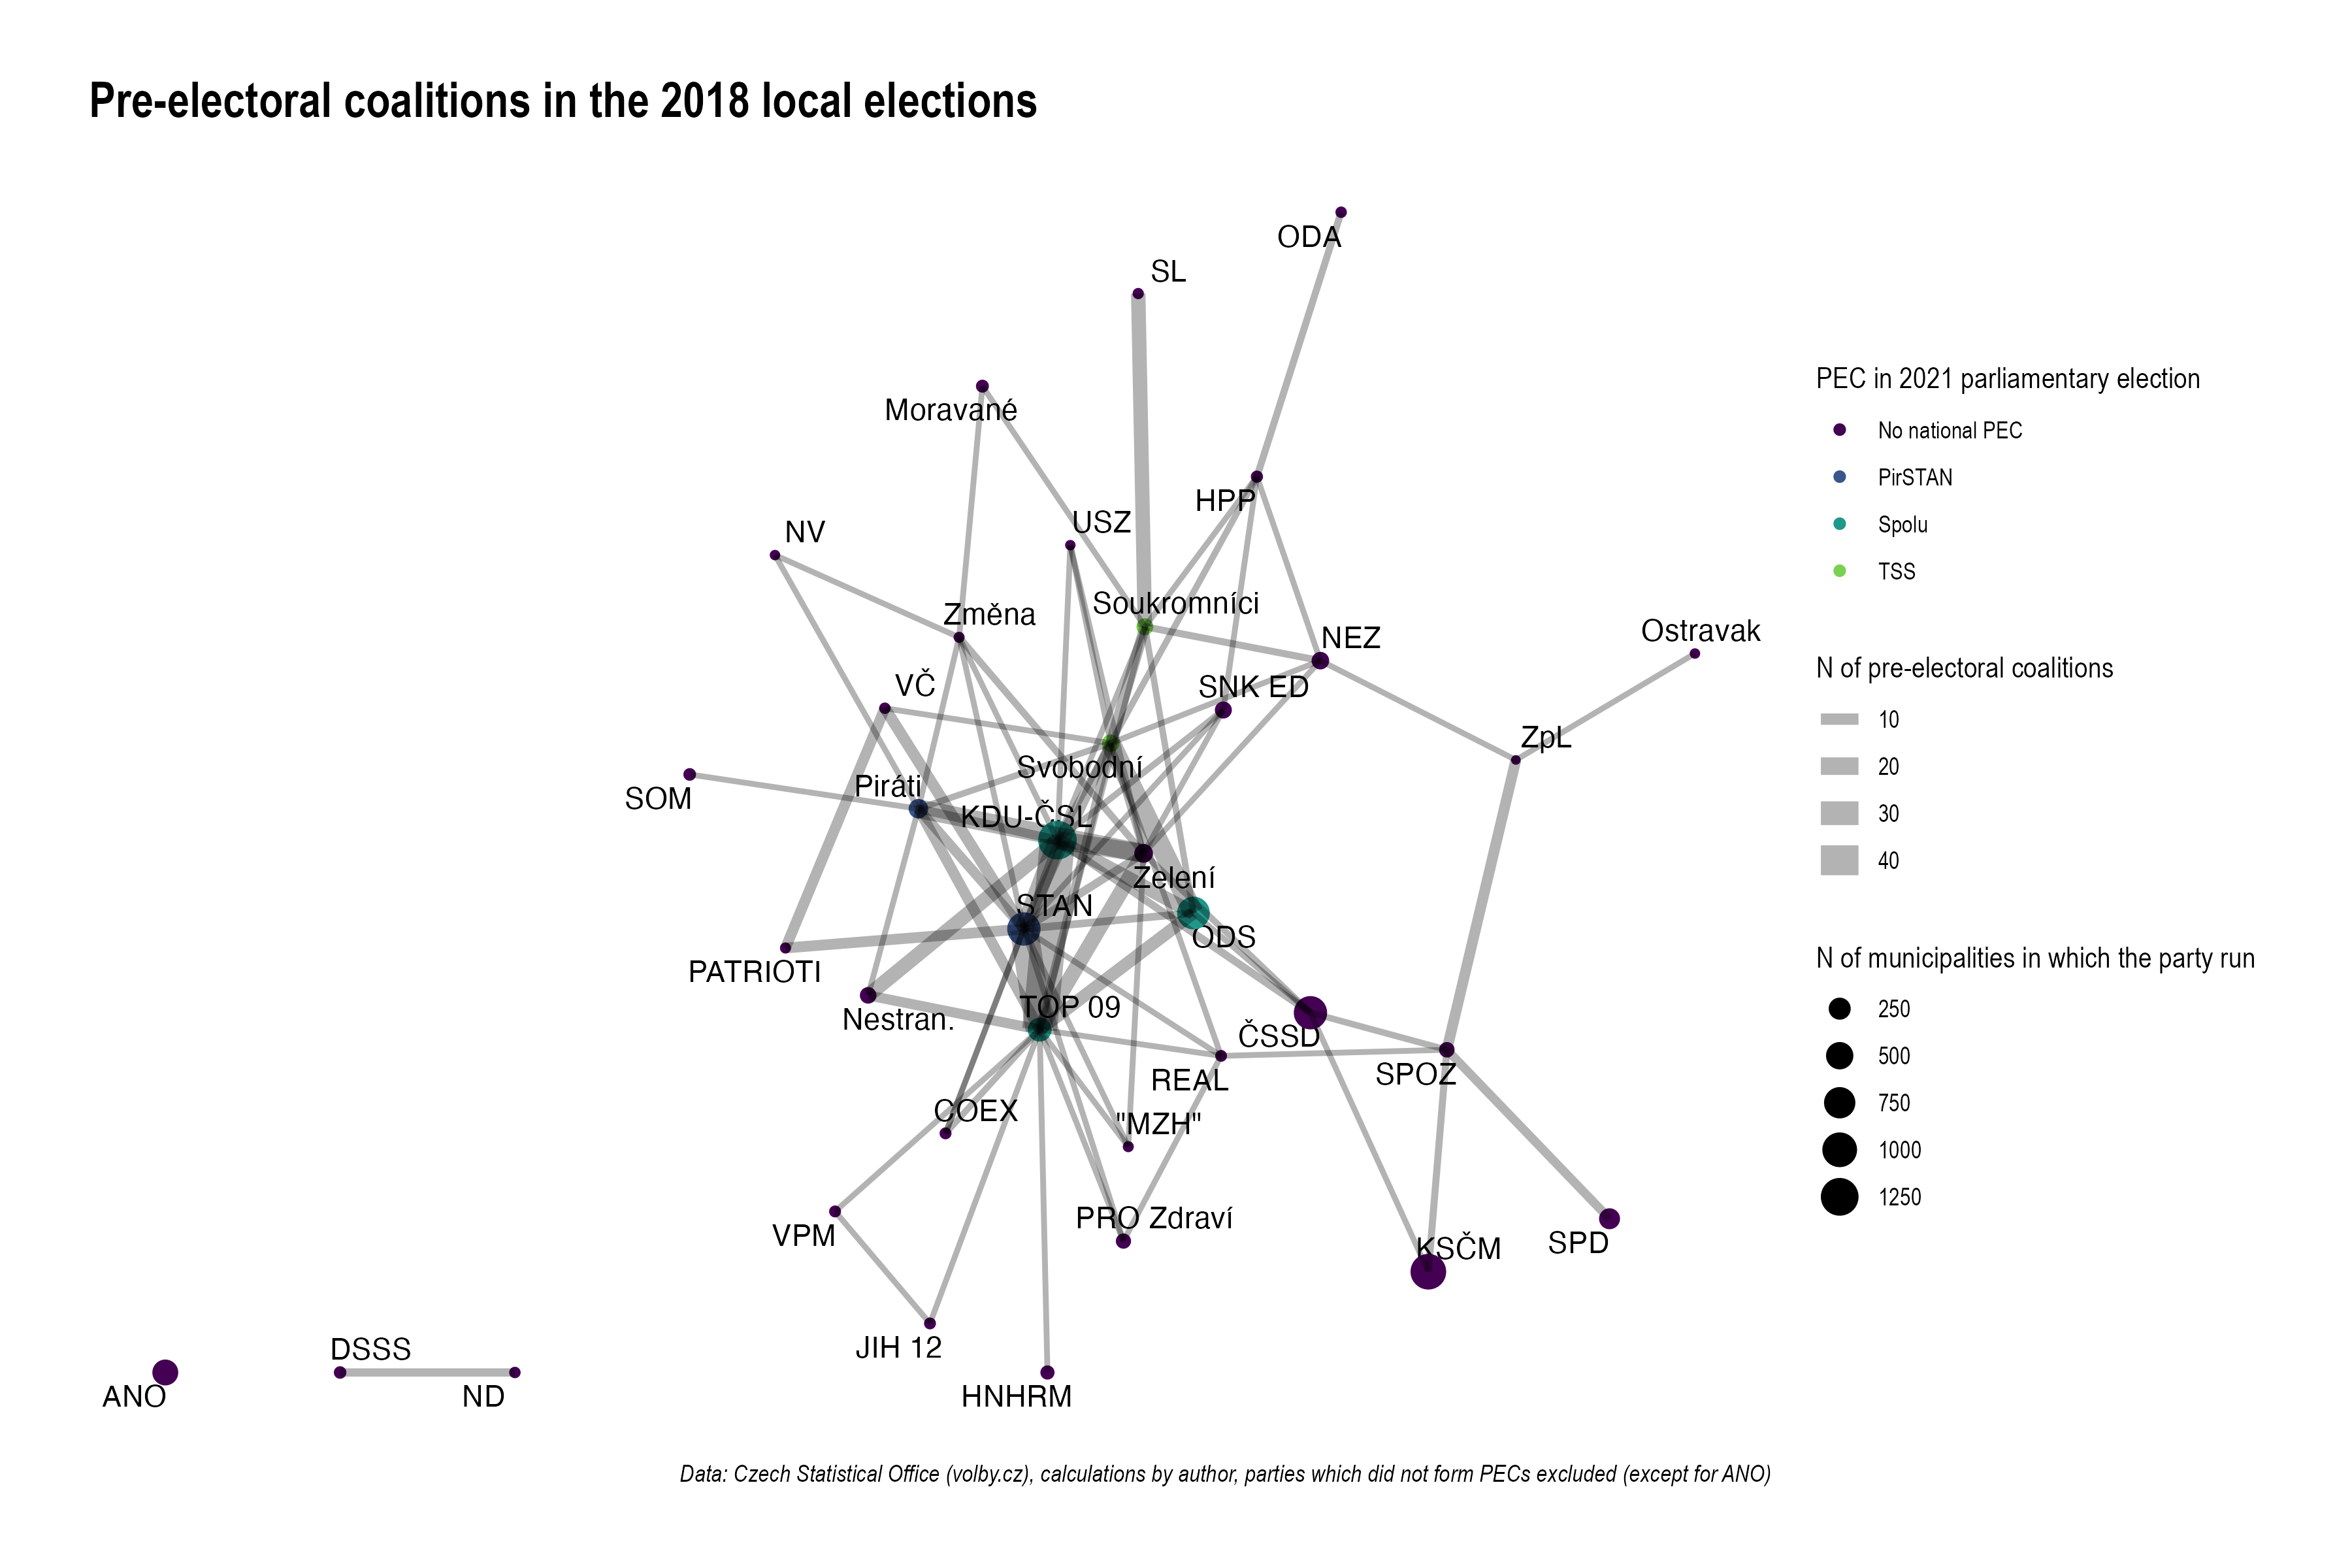
\includegraphics[max size={\textwidth}{\textheight}]{koalice_2018_en.png}
\label{fig:1}
\end{figure}

\begin{figure}[H]
% \centering
\caption{Pre-electoral coalitions in the 2022 local elections}
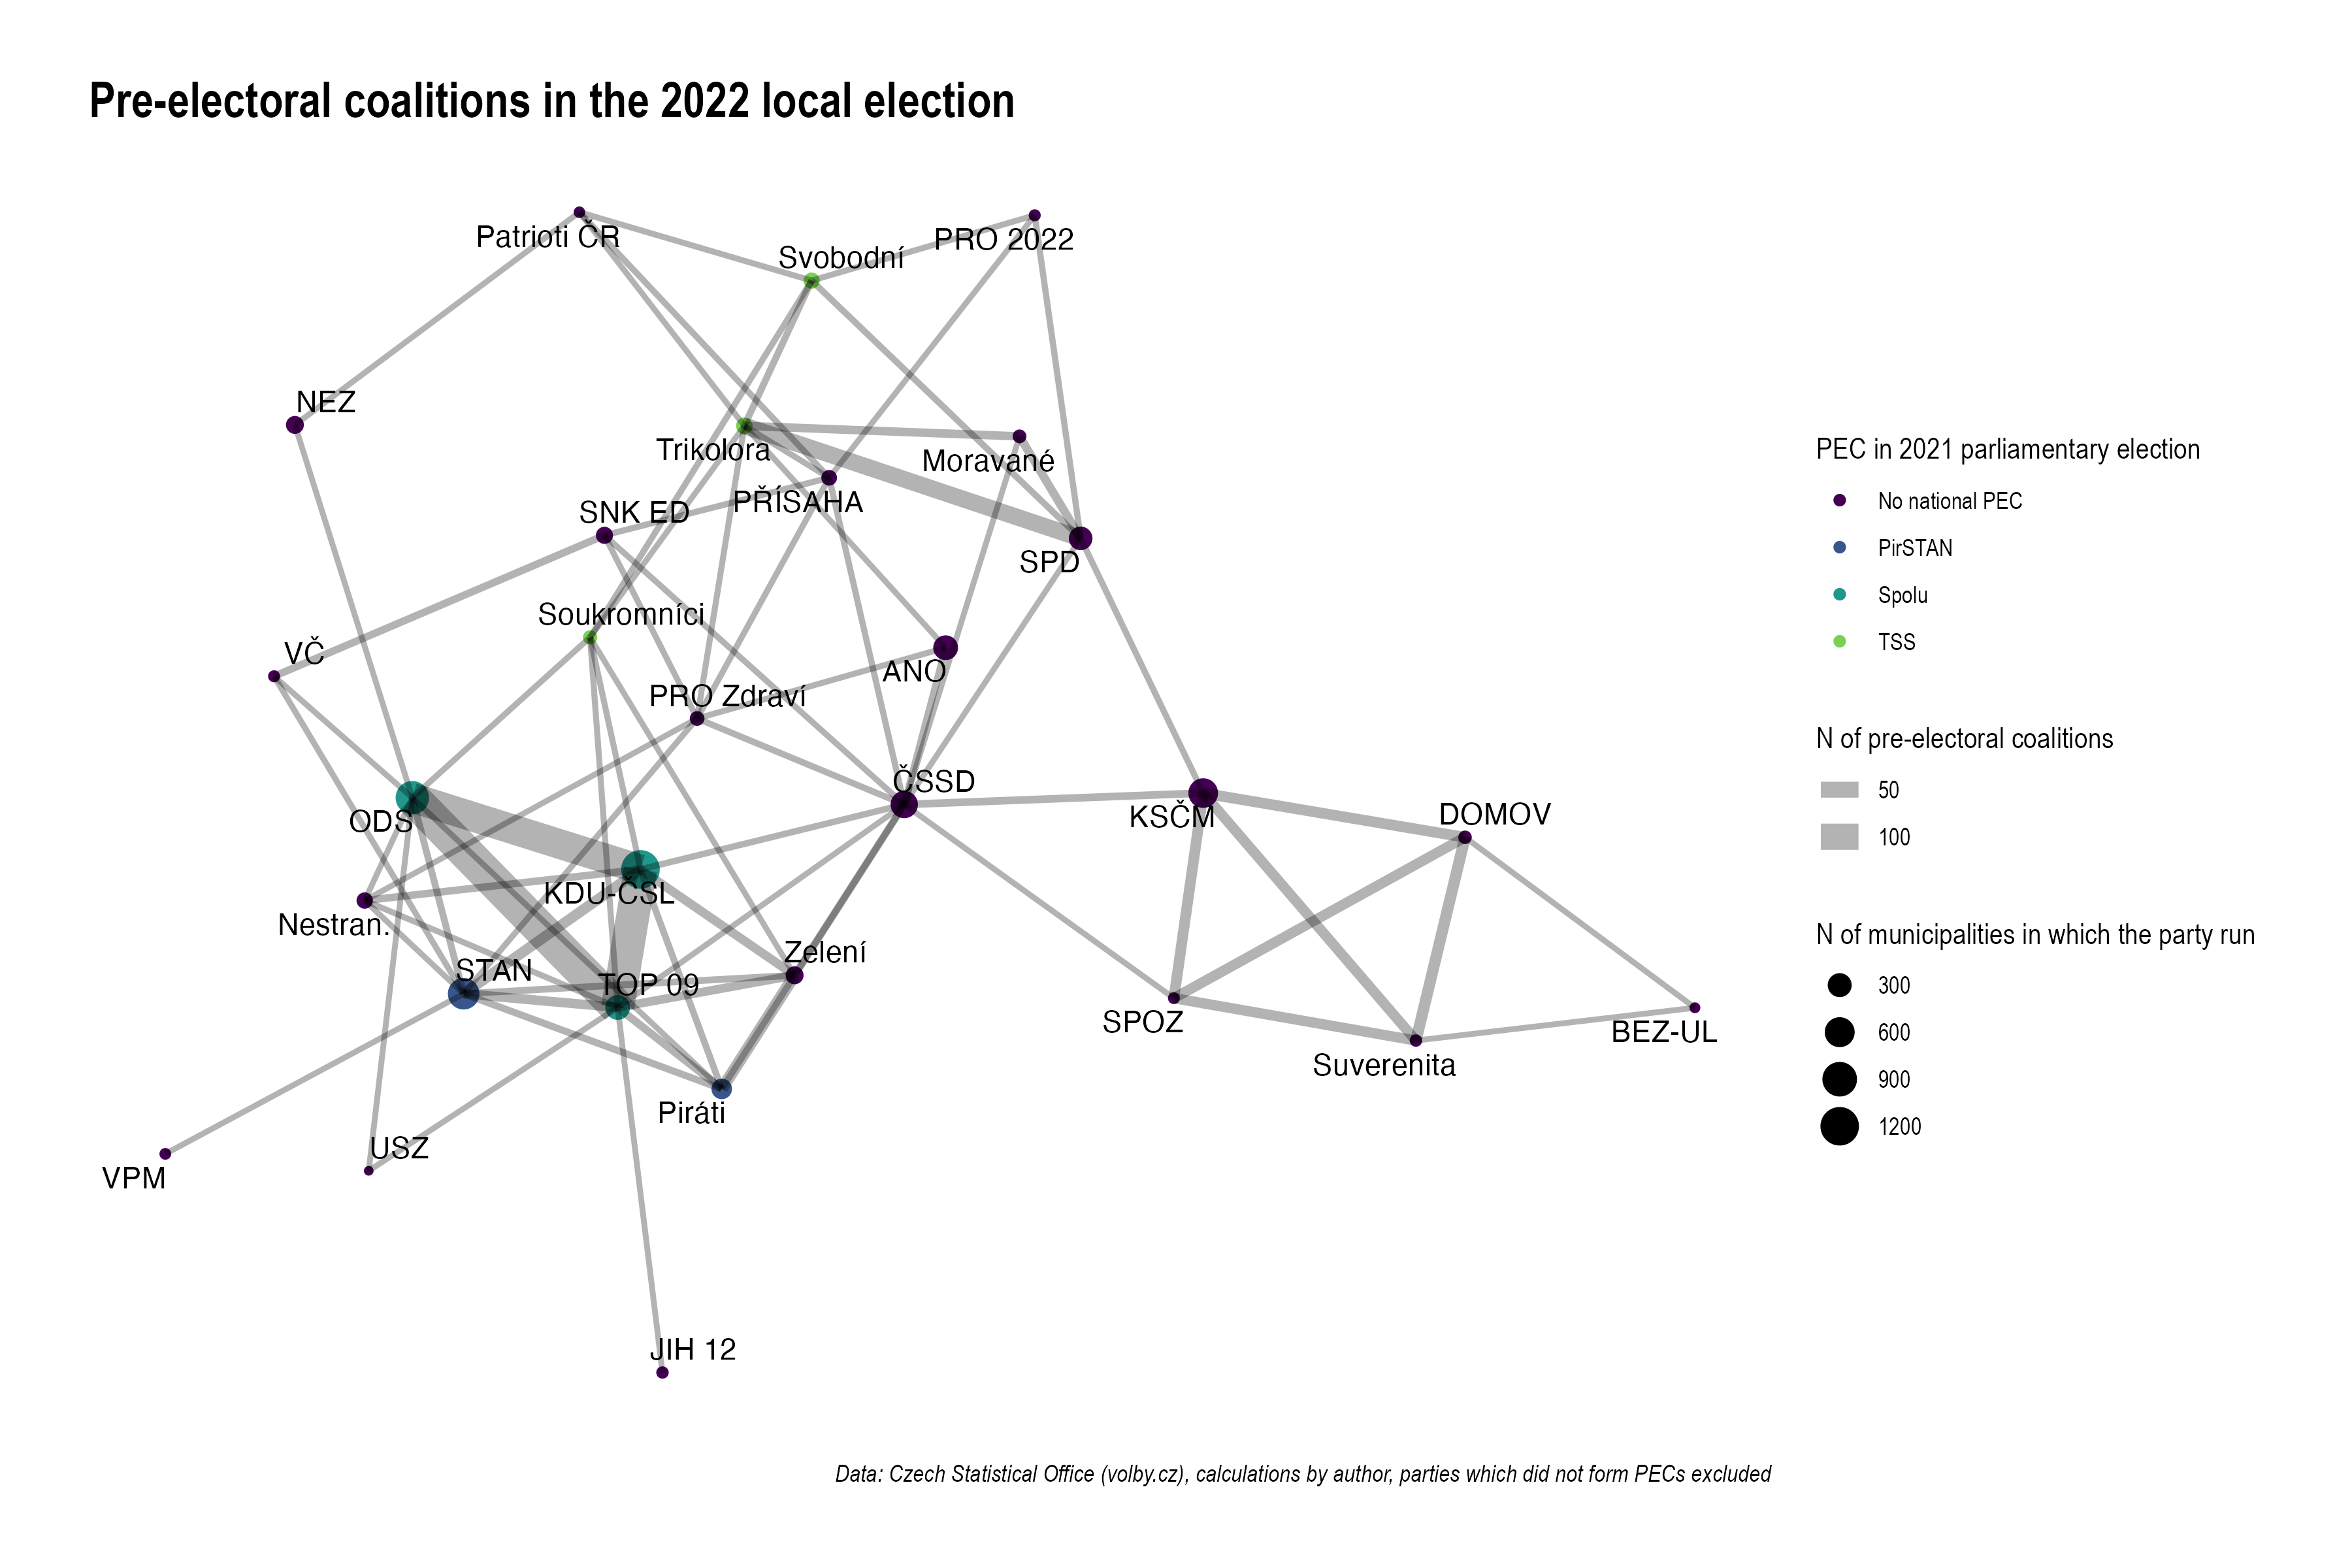
\includegraphics[max size={\textwidth}{\textheight}]{koalice_2022_en.png}
\label{fig:2}
\end{figure}

\section{Results}

In this section, I present the results of the multi-level probit models that explain the formation of a pre-electoral coalition between parties in a dyad, as the models are fitted on the dyadic data. Table \ref{tab:2} displays the estimated models. Additionally, I estimated the same models including a variable measuring ideological distance, which reduces the number of observations due to the unavailability of ideological positions for small and local parties. The results of these models are shown in Table \ref{app:1} in the Appendix. The models in the Appendix yield similar results to those reported below.
% for the ease of interpretation I also present charts with predicted probabilities of pre-electoral coalition formation.

% H1
The first three variables in the models (\emph{Together, PirSTAN} and \emph{TSS}) indicate that the formation of pre-electoral coalitions at the national level had a positive effect on the formation of coalitions at the local in the case of two out of three parties. Specifically, political parties that won the general election under the banner of the Together coalition had the highest probability of forming a coalition (with a predicted probability of around 20\% based on Model 1). Similarly, dyads of the TSS coalition parties were more likely to form a pre-electoral coalition at the local level (with a predicted probability of around 8\%). This finding is somewhat surprising given that TSS garnered only 2.8\% of the votes in the general election and did not enter Parliament. However, local coalitions might still be beneficial due to resource pooling. Finally, the PirSTAN coalition at the national level did not significantly affect the formation of pre-electoral coalitions at the local level, possibly because the coalition underperformed in the national election, candidates from STAN gained majority of the coalition mandates and a conflict between parties ensued whether STAN broke the coalition agreement during the campaign when they allegedly persuaded the voters to cast preferential votes for STAN candidates. All in all, the results support Hypothesis 1.

% H1a
Model 1 also indicates that the electoral success of the national PECs in a given municipality did not significantly increase the probability of creating the same PEC at the local level. As a robustness check, I estimate the same model on a subset of data consisting of dyads between parties that created a national PEC (see \ref{app:2}), which produces the same results. Therefore, these results do not confirm Hypothesis 1a. In consequence, the formation of national PEC in the case of Together and TSS itself was more important for the local elites to follow the suit than their success in a given municipality. 

% Senate PEC
Besides the effect of PEC formation in the general election on the probability of PEC formation at the local level, I also consider the Senate election, the upper chamber of the Czech Parliament. All models indicate that the formation of a pre-electoral coalition in the Senate election in a given district (nominating a joint candidate) is positively associated with the PEC formation by the same parties in municipalities belonging to the district. Therefore, these findings support Hypothesis 2. However, the size of the effect is modest, likely influenced by the proximity of the general election to the local election and the impact of pre-electoral coalitions formed in the general election.
The robustness of this variable's effect was confirmed using matching techniques, which yielded essentially the same results (see Appendix \ref{app:3}).

\begin{table}
\centering
\caption{Models of pre-electoral coalition formation in the 2022 local election \label{tab:2}}
\begin{tabular}[t]{lccccc}
\toprule
& (1) & (2) & (3) & (4) & (5) \\ \midrule 
Together                                & \num{2.03}***  & \num{1.93}***  & \num{1.95}***  & \num{2.03}***  & \num{2.10}***  \\
& (\num{0.43})   & (\num{0.44})   & (\num{0.43})   & (\num{0.43})   & (\num{0.44})   \\
PirSTAN                                 & \num{0.67}     & \num{0.67}     & \num{0.67}     & \num{0.69}     & \num{0.67}     \\
& (\num{0.74})   & (\num{0.74})   & (\num{0.74})   & (\num{0.73})   & (\num{0.74})   \\
TSS                                     & \num{1.33}*    & \num{1.34}*    & \num{1.33}*    & \num{1.34}*    & \num{1.35}*    \\
& (\num{0.54})   & (\num{0.54})   & (\num{0.54})   & (\num{0.54})   & (\num{0.54})   \\
Vote share change in GE                 & \num{0.03}    & \num{0.04}    & \num{0.03}    & \num{0.04}    & \num{0.03}     \\
& (\num{0.02})   & (\num{0.02})   & (\num{0.02})   & (\num{0.02})   & (\num{0.02})   \\
Senate PEC (2022)                       & \num{0.29}*    & \num{0.29}*    & \num{0.34}**   & \num{0.29}*    & \num{0.31}**   \\
& (\num{0.12})   & (\num{0.12})   & (\num{0.12})   & (\num{0.12})   & (\num{0.12})   \\
ANO in local government                 &                 & \num{0.05}     &                 &                 &                 \\
&                 & (\num{0.09})   &                 &                 &                 \\
Together × ANO in local gov.            &                 & \num{0.24}    &                 &                 &                 \\
&                 & (\num{0.13})   &                 &                 &                 \\
KSČM in local government                &                 &                 & \num{0.05}     &                 &                 \\
&                 &                 & (\num{0.13})   &                 &                 \\
Together × KSČM in local gov.           &                 &                 & \num{0.71}**   &                 &                 \\
&                 &                 & (\num{0.22})   &                 &                 \\
Same local gov. position                &                 &                 &                 & \num{0.27}***  &                 \\
&                 &                 &                 & (\num{0.07})   &                 \\
Local gov. position: Both in government &                 &                 &                 &                 & \num{-0.23}   \\
&                 &                 &                 &                 & (\num{0.12})   \\
Local gov. position: Both in opposition &                 &                 &                 &                 & \num{0.39}***  \\
&                 &                 &                 &                 & (\num{0.07})   \\
Controls & Yes & Yes & Yes & Yes & Yes \\
\midrule
N                                & \num{13266}    & \num{13266}    & \num{13266}    & \num{13266}    & \num{13266}    \\
R2 Marg.                                & \num{0.239}    & \num{0.238}    & \num{0.240}    & \num{0.249}    & \num{0.258}    \\
R2 Cond.                                & \num{0.520}    & \num{0.520}    & \num{0.518}    & \num{0.523}    & \num{0.531}    \\
AIC                                     & \num{3018.7}   & \num{3017.2}   & \num{3007.7}   & \num{3003.7}   & \num{2977.0}   \\
BIC                                     & \num{3116.1}   & \num{3129.6}   & \num{3120.0}   & \num{3108.6}   & \num{3089.4}   \\
ICC                                     & \num{0.4}      & \num{0.4}      & \num{0.4}      & \num{0.4}      & \num{0.4}      \\
\bottomrule
\multicolumn{6}{l}{\rule{0pt}{1em}* p $<$ 0.05, ** p $<$ 0.01, *** p $<$ 0.001}\\
\end{tabular}
\end{table}


When comparing the effect sizes of pre-electoral coalitions in the general election—particularly the Together and TSS coalitions—and PECs in the Senate election, we see that PECs in the general election had a much larger impact than PECs in the Senate election. This difference can be attributed to the general election being 'first-order' in the Czech political system, where the electoral advantage of PECs was well-known, unlike the Senate election which was concurrent with the local election. The only known advantage is that the parties forming pre-electoral coalitions in the Senate election could benefit from pooling resources in the campaign. Moreover, the political investments made to create PECs in the general election likely influenced their formation in the Senate and local elections. In retrospect, the Together coalition invested significant political capital in maintaining its coalition, evidenced by its pursuit of joint candidates not only in the Senate and local elections but also in creating a joint list for the 2024 European Parliament elections, despite its constituent parties belonging to different euro-parties\footnote{ODS belongs to ECR, while KDU-ČSL and TOP 09 belongs to EPP.}. The inclusion of the Senate PEC formation in the models slightly decreases the effect of Together coalition, suggesting that the effect of national PEC is partly mediated by the creation of Senate PECs.

% Hyp 3a and 3b
% ANO in local government
Next, I turn to the hypotheses related to electoral competition in local elections. If electoral competition were shaped by a logic similar to that seen in the 2021 general election, we might expect the Together coalition to be more likely in municipalities where ANO participates in local government. However, Model 2 in Table \ref{tab:2} shows that the effect of the interaction \emph{Together} $\times$ \emph{ANO in local government} is rather small and statistically insignificant. While the interaction \emph{Together} $\times$ \emph{KSČM in local government} is positive and statistically significant, Figure \ref{fig:3} indicates that the confidence intervals for Together coalition dyads overlap. Therefore, the results do not support either Hypothesis 3a or 3b.

The results show that the strength of populist parties does not induce other parties to form PECs at the local level. This, however, does not necessarily mean that populist/anti-populist divide does not influence elections at all. Instead, populist/anti-populist divide explains which parties coalesce together as models using distance between parties show (see Appendix \ref{app:1}). Specifically, the greater the difference in parties' positions on the anti-elite scale, the less likely they are to form a PEC.

\begin{figure}[H]
% \centering
\caption{Interaction between Together PEC formation and local government}
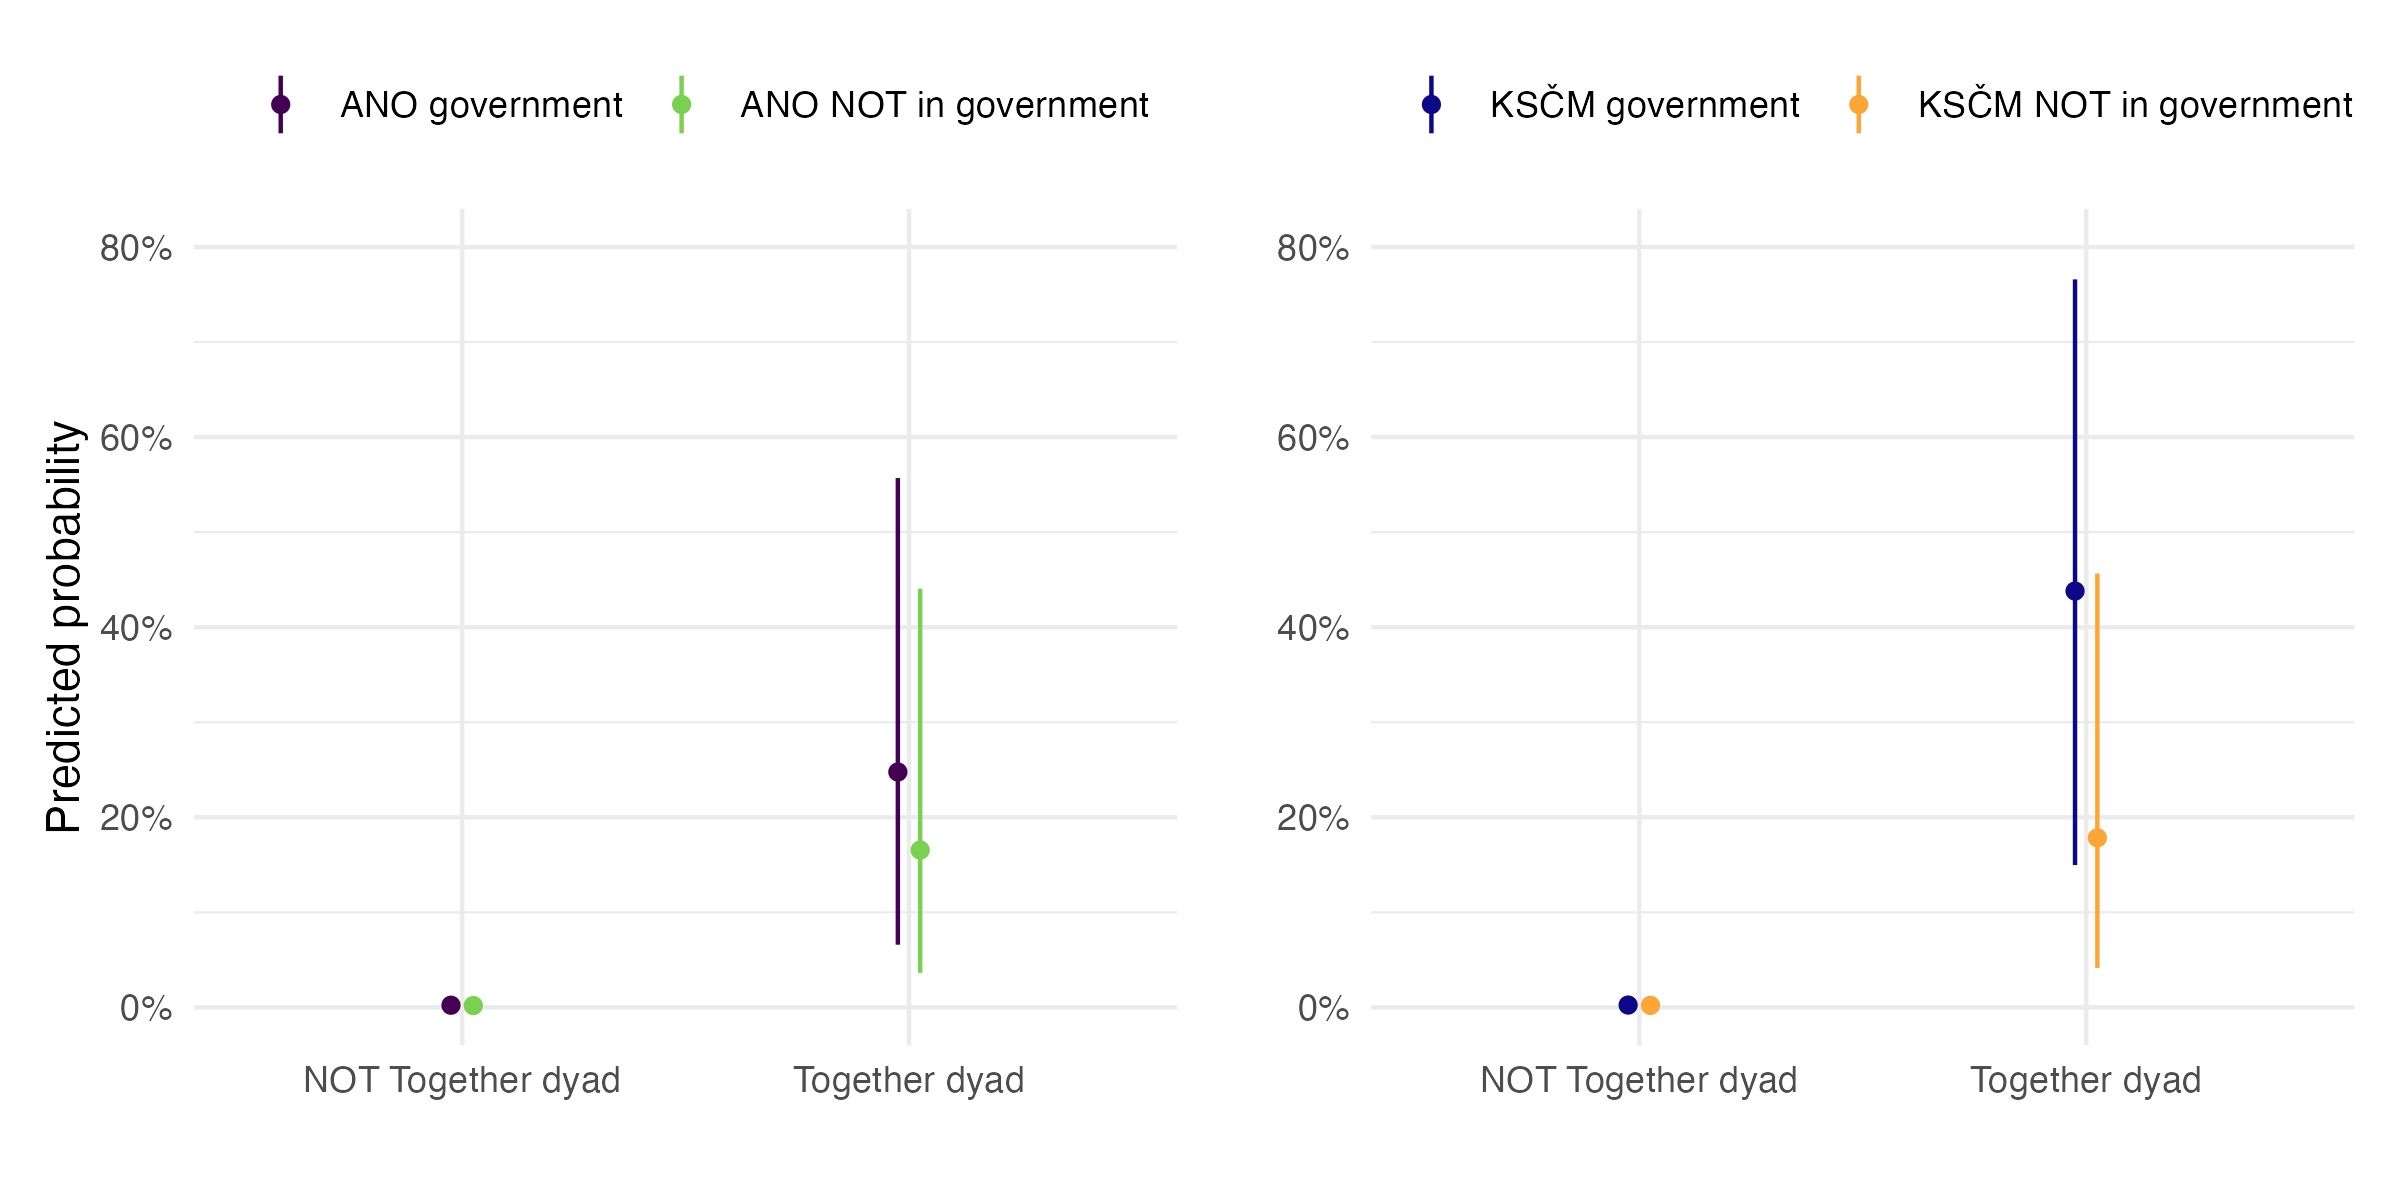
\includegraphics[max size={\textwidth}{\textheight}]{gov_interaction.png}
\label{fig:3}
\end{figure}

% Same local gov. position
Finally, we examine the impact of parties' positions in local government on the probability of coalition formation, as formulated in Hypothesis 4. Model 4 in Table \ref{tab:2} demonstrates this relationship. The effect of holding the same position in local government is positive and statistically significant, although the size of the effect is relatively small. Nevertheless, Hypothesis 4 is supported. Additionally, Model 5 distinguishes between both parties being in the local government and both in the opposition with different positions as a baseline category. It shows that the parties are more likely to form a PEC if they both are in the opposition. Overall, the results concerning parties' positions in local government highlight the significant role of local concerns and ambitions in pre-electoral coalition formation at the local level. Apart from following the patterns of electoral competition from the national level, local party branches coalesce to improve their position for the post-election government negotiations.


\section{Conclusion}

The 2021 general election reshaped the Czech party system and also influenced party competition in many municipalities. Notably, the Together coalition, which won in the parliamentary election followed suit in the local election and formed pre-electoral coalitions at the local level. The same is true for the TSS pre-electoral coalition formed by three minor parties, which somewhat overperformed in the general election but failed to gain representation in Parliament. In contrast, the last pre-electoral coalition, the Pirates and the Mayors and Independents, which underperformed in the general election did not form the same pre-electoral coalitions at the local level. 

Besides the general election, the formation of pre-electoral coalitions for the Senate election, which took place concurrently with the local election marginally increases the probability of pre-electoral coalition formation at the local level. The effect is much smaller than in the case of a general election, which is understandable as the only benefit the Senate election could bring to the parties is pooling resources during the campaign.

Unlike the Senate election, the general election could provide a testing ground for the coalitions from which the local branches could learn if forming such a coalition is beneficial. Surprisingly, the probability of forming the same PEC at the local level is not related to the PEC's electoral gain in the general election in a given municipality. This suggests that the national performance and the political capital invested in forming the coalitions at the national level overshadowed local-level electoral benefits. After all, the benefits of both the Together and TSS coalitions, which were more likely to form during the local election, were predominantly positive. Only in 4.6\% of municipalities included in this study did the Together coalition gain a lower vote share in 2021 than in the 2017 general election. In the case of TSS, they benefited everywhere.

In contrast to the 2021 general election, when the right-wing parties created the Together coalition to oust the populist ANO from the government, the contextual effect of ANO local government on the probability of forming the Together coalition at the local level is inconclusive. This challenges the theoretical expectation that pre-electoral coalitions are more likely to emerge if they face more extreme government alternatives as the creation of the Together coalition was not more likely if they faced ANO. This outcome may suggest that the populist/anti-populist is not extreme enough. Additionally, the lack of effect may result from the fact that not all pre-electoral coalitions are equal. The research on pre-electoral coalitions combined all of its forms, yet the likelihood of pre-electoral coalition formation may differ across different contexts. For instance, pre-electoral coalitions in the form of supporting a candidate in the second round of a two-round electoral system may be more likely to emerge if they face a far-right opponent (see, for example, the strategic withdrawal of centre and left-wing candidates from the race during the 2024 French parliamentary election). However, this may not be true for pre-electoral coalitions in the form of joint party lists in PR electoral systems. 

Instead, the results indicate that the formation of PECs is motivated by an attempt to replace not only ANO but any other party. This does not concern only the Together coalition; the formation of a pre-electoral coalition was more likely between parties in the same position in local government. This suggests that the spill-over is dependent on local conditions. 

Although this paper contributes empirical evidence on the spill-over, some party properties were left out of the analysis and can be considered as avenues for future research. For instance, party centralization may increase the probability that the national PECs permeate to the local level. Unfortunately, in this case, in all studied parties, local branches are responsible for candidate selection for the municipal election, so the effect of centralization cannot be estimated. Nevertheless, our case indicates that despite the lack of centralization, the local branches followed suit when creating PECs at the local level. 

\bibliographystyle{tfcad}
\bibliography{bibliography}

\newpage
\appendix

\section{Dyads}

\begin{figure}[H]
% \centering
\caption{Created local PECs in dyads}
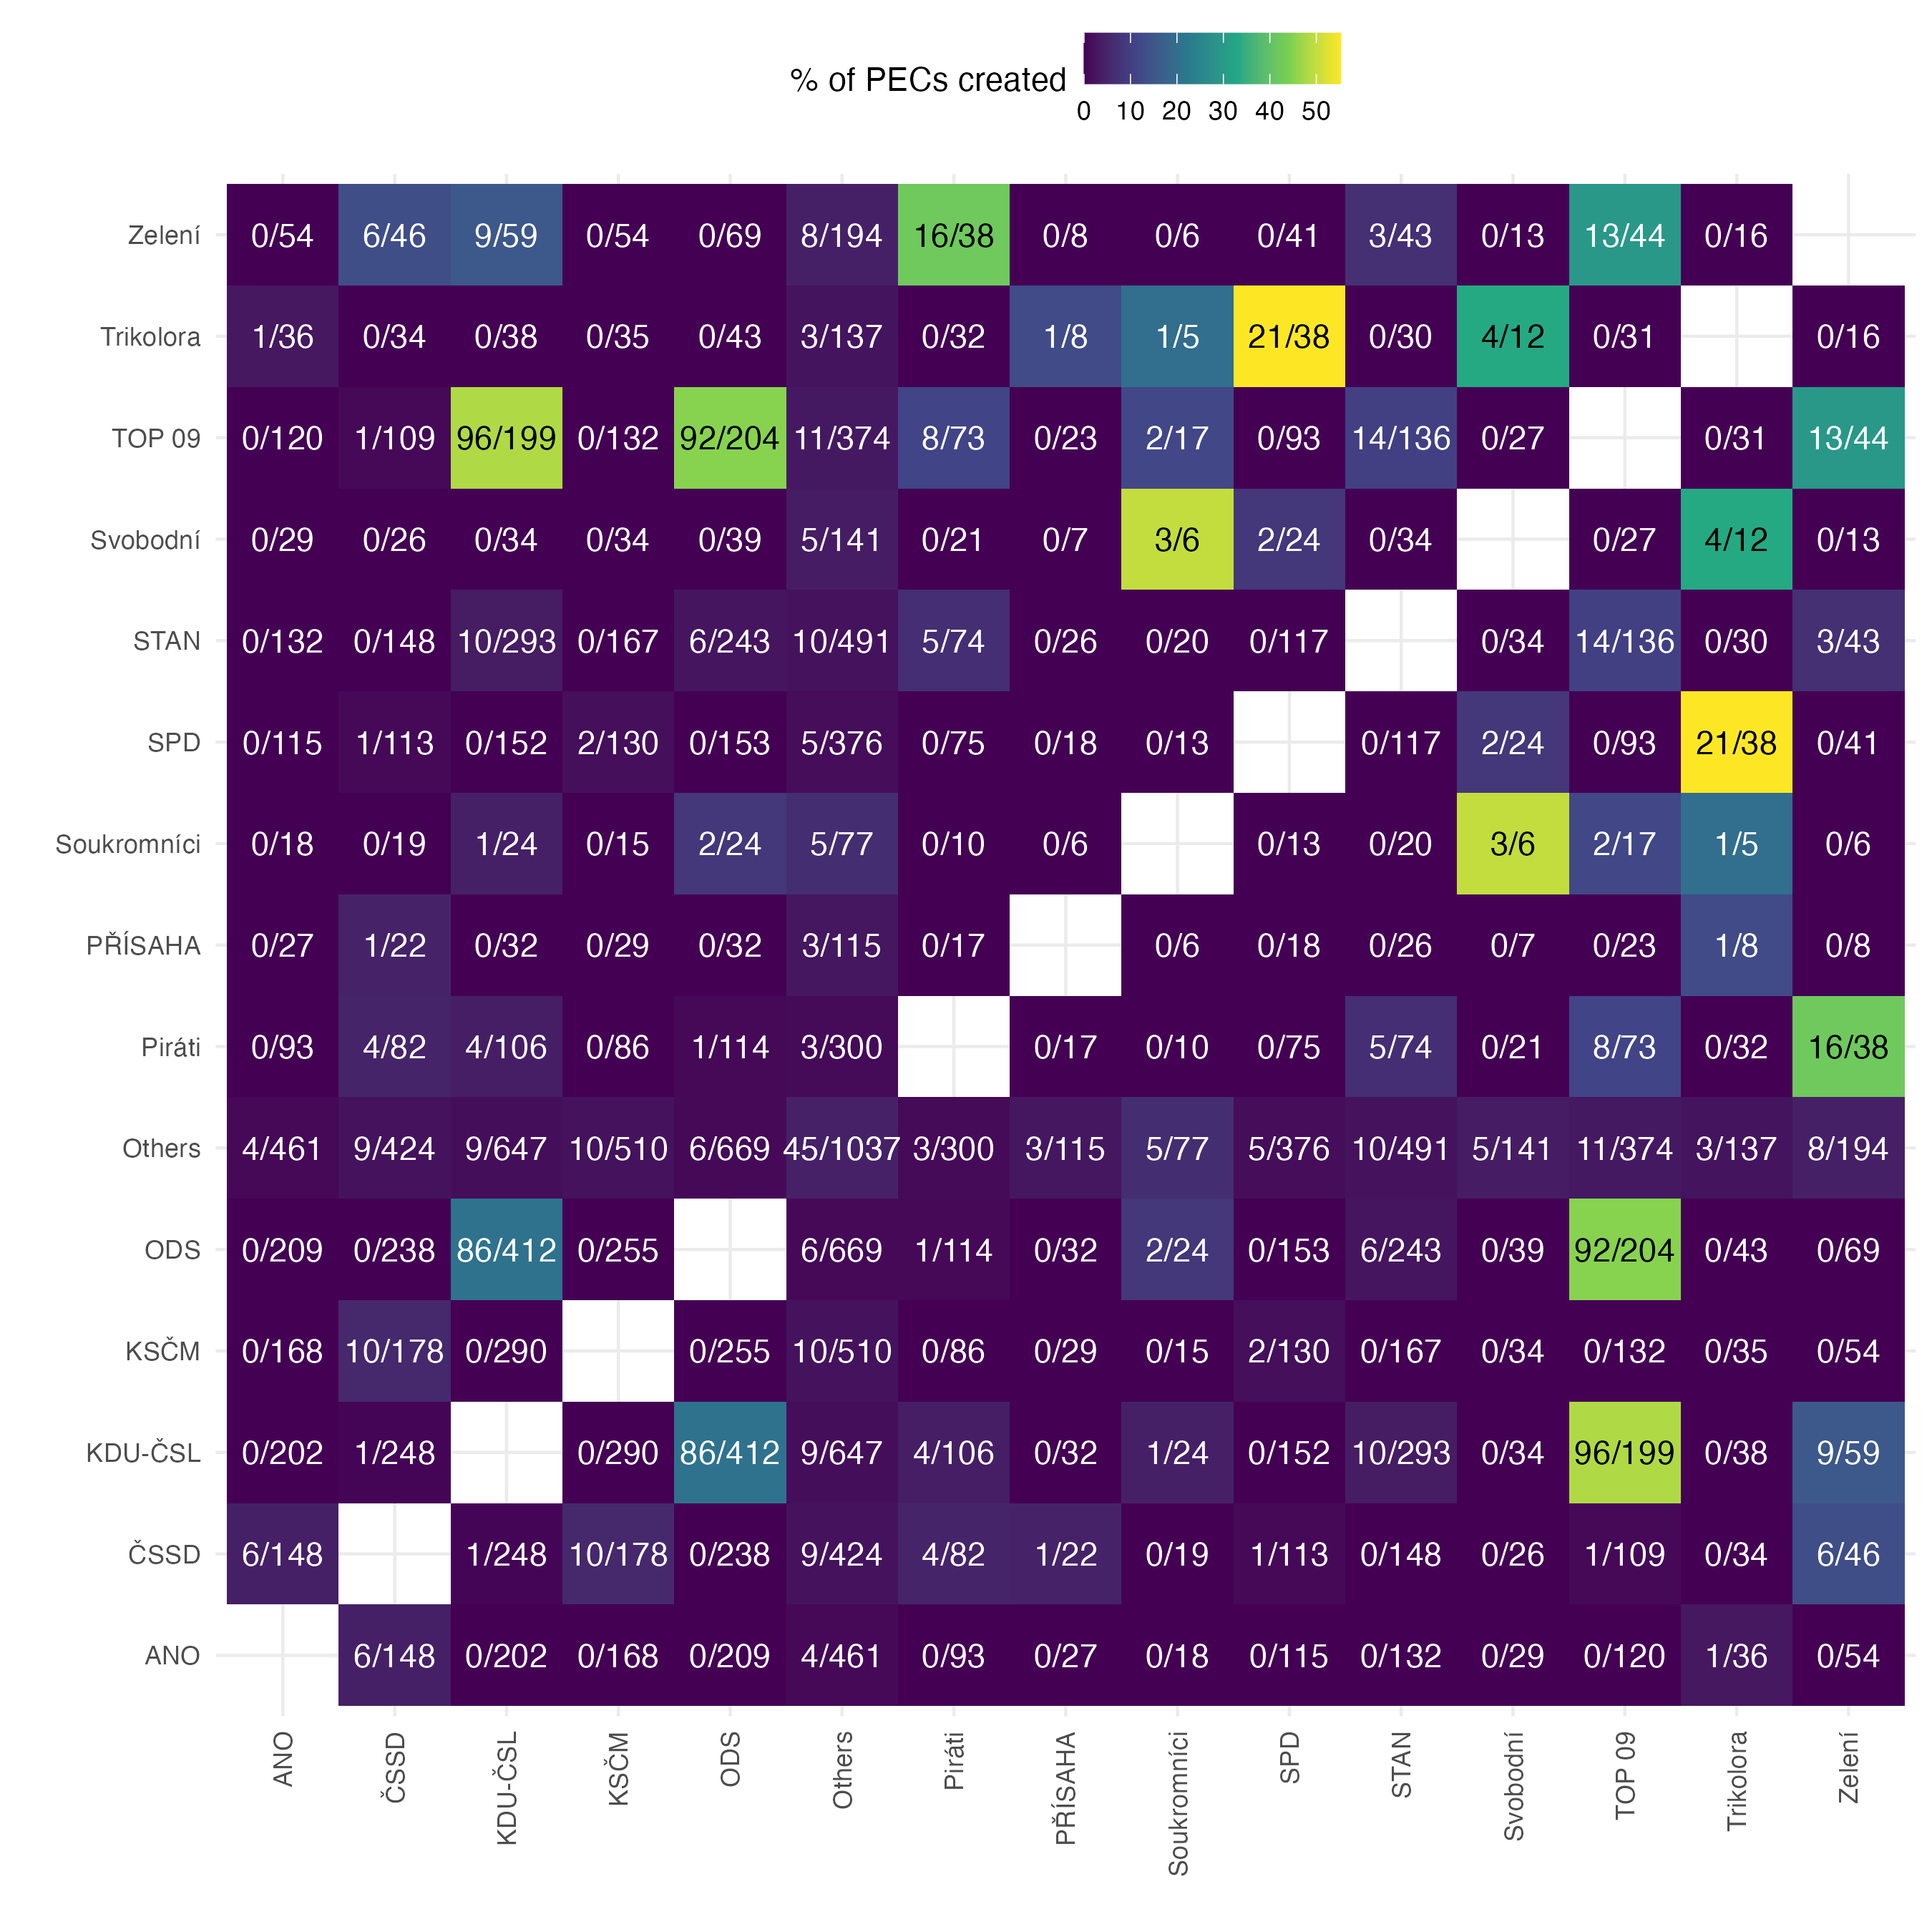
\includegraphics[max size={\textwidth}{\textheight}]{dyad_heatmap.png}
\begin{minipage}{5.5in}
\footnotesize{Note: The numbers in cells indicate how many times the parties formed a pre-electoral coalition out of all posible cases (municipalities in which they both run)}
\end{minipage}
\label{fig:a1}
\end{figure}

\begin{figure}[H]
% \centering
\caption{Created Senate PECs in dyads}
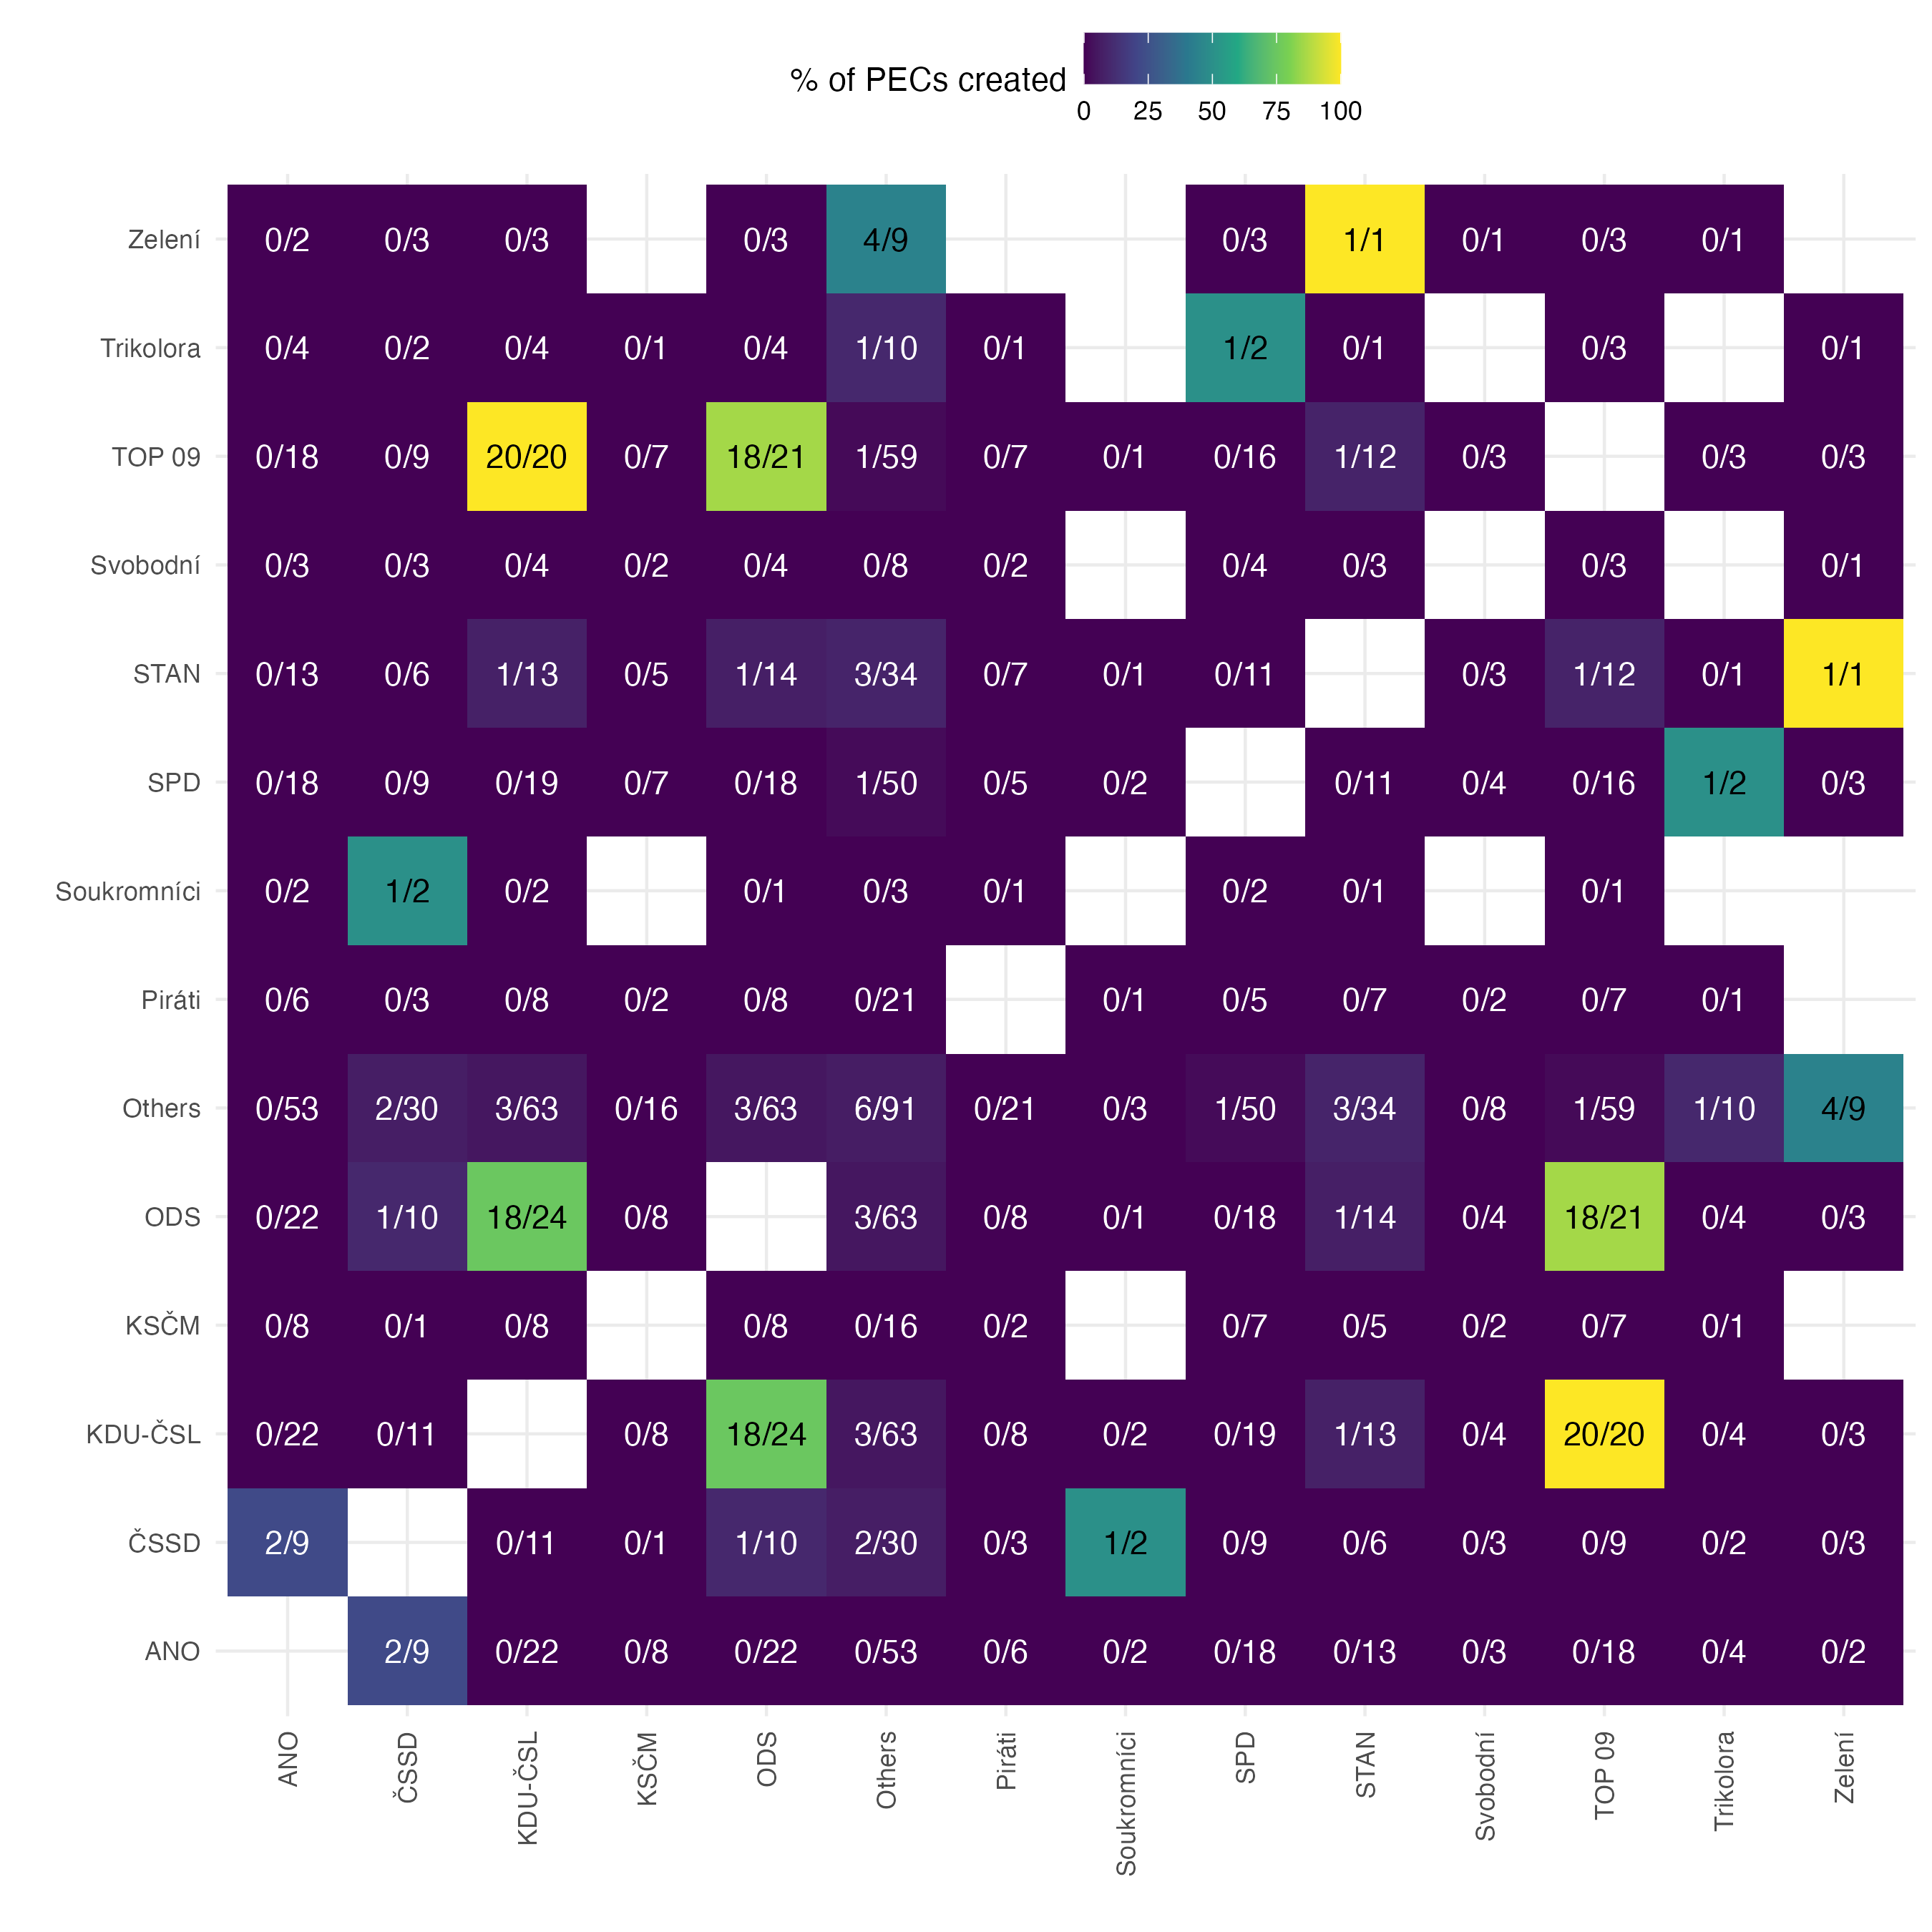
\includegraphics[max size={\textwidth}{\textheight}]{senate_dyad_heatmap.png}
\begin{minipage}{5.5in}
\footnotesize{Note: The numbers in cells indicate how many times the parties formed a pre-electoral coalition out of all posible cases (Senate districts in which they both run)}
\end{minipage}
\label{fig:a2}
\end{figure}

\newpage

\section{Full Models}
\begin{table}[!h]
\centering
\begin{adjustbox}{max width=6in}
\begin{tabular}[t]{lccccc}
\toprule
  & (1) & (2) & (3) & (4) & (5) \\
\midrule
Together                                & \num{2.03}***  & \num{1.93}***  & \num{1.95}***  & \num{2.03}***  & \num{2.10}***  \\
& (\num{0.43})   & (\num{0.44})   & (\num{0.43})   & (\num{0.43})   & (\num{0.44})   \\
PirSTAN                                 & \num{0.67}     & \num{0.67}     & \num{0.67}     & \num{0.69}     & \num{0.67}     \\
& (\num{0.74})   & (\num{0.74})   & (\num{0.74})   & (\num{0.73})   & (\num{0.74})   \\
TSS                                     & \num{1.33}*    & \num{1.34}*    & \num{1.33}*    & \num{1.34}*    & \num{1.35}*    \\
& (\num{0.54})   & (\num{0.54})   & (\num{0.54})   & (\num{0.54})   & (\num{0.54})   \\
Vote share change in GE                 & \num{0.03}    & \num{0.04}    & \num{0.03}    & \num{0.04}    & \num{0.03}     \\
& (\num{0.02})   & (\num{0.02})   & (\num{0.02})   & (\num{0.02})   & (\num{0.02})   \\
Senate PEC (2022)                       & \num{0.29}*    & \num{0.29}*    & \num{0.34}**   & \num{0.29}*    & \num{0.31}**   \\
& (\num{0.12})   & (\num{0.12})   & (\num{0.12})   & (\num{0.12})   & (\num{0.12})   \\
ANO in local government                 &                 & \num{0.05}     &                 &                 &                 \\
&                 & (\num{0.09})   &                 &                 &                 \\
Together × ANO in local gov.            &                 & \num{0.24}    &                 &                 &                 \\
&                 & (\num{0.13})   &                 &                 &                 \\
KSČM in local government                &                 &                 & \num{0.05}     &                 &                 \\
&                 &                 & (\num{0.13})   &                 &                 \\
Together × KSČM in local gov.           &                 &                 & \num{0.71}**   &                 &                 \\
&                 &                 & (\num{0.22})   &                 &                 \\
Same local gov. position                &                 &                 &                 & \num{0.27}***  &                 \\
&                 &                 &                 & (\num{0.07})   &                 \\
Local gov. position: Both in government &                 &                 &                 &                 & \num{-0.23}   \\
&                 &                 &                 &                 & (\num{0.12})   \\
Local gov. position: Both in opposition &                 &                 &                 &                 & \num{0.39}***  \\
&                 &                 &                 &                 & (\num{0.07})   \\
Local PEC (2018)                        & \num{2.14}***  & \num{2.13}***  & \num{2.13}***  & \num{2.03}***  & \num{2.12}***  \\
& (\num{0.14})   & (\num{0.14})   & (\num{0.14})   & (\num{0.14})   & (\num{0.15})   \\
Coalition size                          & \num{-0.43}*** & \num{-0.43}*** & \num{-0.43}*** & \num{-0.41}*** & \num{-0.33}*** \\
& (\num{0.04})   & (\num{0.04})   & (\num{0.04})   & (\num{0.04})   & (\num{0.04})   \\
Asymmetry                               & \num{-0.07}    & \num{-0.07}    & \num{-0.08}    & \num{-0.03}    & \num{-0.03}    \\
& (\num{0.16})   & (\num{0.17})   & (\num{0.16})   & (\num{0.17})   & (\num{0.17})   \\
ENEP                                    & \num{-0.06}*** & \num{-0.07}*** & \num{-0.06}*** & \num{-0.06}**  & \num{-0.05}**  \\
& (\num{0.02})   & (\num{0.02})   & (\num{0.02})   & (\num{0.02})   & (\num{0.02})   \\
Coalition size × asymmetry              & \num{0.20}**   & \num{0.19}*    & \num{0.20}**   & \num{0.20}**   & \num{0.16}*    \\
& (\num{0.07})   & (\num{0.07})   & (\num{0.07})   & (\num{0.08})   & (\num{0.08})   \\
Intercept                             & \num{-1.60}*** & \num{-1.55}*** & \num{-1.60}*** & \num{-1.87}*** & \num{-2.08}*** \\
& (\num{0.17})   & (\num{0.17})   & (\num{0.17})   & (\num{0.18})   & (\num{0.19})   \\
\midrule
Municipality-level variance             & \num{0.12}     & \num{0.12}     & \num{0.11}     & \num{0.11}     & \num{0.11}     \\
Dyad-level variance                     & \num{0.47}     & \num{0.47}     & \num{0.46}     & \num{0.46}     & \num{0.47}     \\
N municipalities                        & \num{1058}  & \num{1058}  & \num{1058}  & \num{1058}  & \num{1058}  \\
N party dyads                           & \num{106}   & \num{106}   & \num{106}   & \num{106}   & \num{106}   \\
N observations                          & \num{13266}    & \num{13266}    & \num{13266}    & \num{13266}    & \num{13266}    \\
R2 Marg.                                & \num{0.239}    & \num{0.238}    & \num{0.240}    & \num{0.249}    & \num{0.258}    \\
R2 Cond.                                & \num{0.520}    & \num{0.520}    & \num{0.518}    & \num{0.523}    & \num{0.531}    \\
AIC                                     & \num{3018.7}   & \num{3017.2}   & \num{3007.7}   & \num{3003.7}   & \num{2977.0}   \\
BIC                                     & \num{3116.1}   & \num{3129.6}   & \num{3120.0}   & \num{3108.6}   & \num{3089.4}   \\
ICC                                     & \num{0.4}      & \num{0.4}      & \num{0.4}      & \num{0.4}      & \num{0.4}      \\
\bottomrule
\multicolumn{6}{l}{\rule{0pt}{1em}* p $<$ 0.05, ** p $<$ 0.01, *** p $<$ 0.001}\\
\end{tabular}

\end{adjustbox}
\end{table}

\newpage

\section{Robustness check: Models with ideological distance}
\label{app:1}
\begin{table}[!h]
\centering
\begin{adjustbox}{max width=5.5in}
\begin{tabular}[t]{lccccc}
\toprule
  & (1) & (2) & (3) & (4) & (5) \\
\midrule

Together                                & \num{1.63}**   & \num{1.45}*    & \num{1.36}*    & \num{1.63}**   & \num{1.70}**   \\
& (\num{0.57})   & (\num{0.58})   & (\num{0.58})   & (\num{0.56})   & (\num{0.57})   \\
PirSTAN                                 & \num{0.69}     & \num{0.72}     & \num{0.71}     & \num{0.72}     & \num{0.71}     \\
& (\num{0.89})   & (\num{0.90})   & (\num{0.90})   & (\num{0.88})   & (\num{0.89})   \\
Vote share change in GE                 & \num{0.03}     & \num{0.04}     & \num{0.04}     & \num{0.03}     & \num{0.03}     \\
& (\num{0.02})   & (\num{0.02})   & (\num{0.02})   & (\num{0.02})   & (\num{0.02})   \\
Senate PEC (2022)                       & \num{0.22}     & \num{0.22}     & \num{0.28}*    & \num{0.21}     & \num{0.23}    \\
& (\num{0.14})   & (\num{0.14})   & (\num{0.14})   & (\num{0.14})   & (\num{0.14})   \\
ANO in local government                 &                 & \num{-0.06}    & \num{-0.05}    &                 &                 \\
&                 & (\num{0.14})   & (\num{0.14})   &                 &                 \\
Together × ANO in local gov.            &                 & \num{0.40}*    & \num{0.38}*    &                 &                 \\
&                 & (\num{0.17})   & (\num{0.17})   &                 &                 \\
KSČM in local government                &                 &                 & \num{-0.16}    &                 &                 \\
&                 &                 & (\num{0.23})   &                 &                 \\
Together × KSČM in local gov.           &                 &                 & \num{0.97}**   &                 &                 \\
&                 &                 & (\num{0.30})   &                 &                 \\
Same local gov. position                &                 &                 &                 & \num{0.37}***  &                 \\
&                 &                 &                 & (\num{0.09})   &                 \\
Local gov. position: Both in government &                 &                 &                 &                 & \num{-0.12}    \\
&                 &                 &                 &                 & (\num{0.14})   \\
Local gov. position: Both in opposition &                 &                 &                 &                 & \num{0.56}***  \\
&                 &                 &                 &                 & (\num{0.10})   \\
Local PEC (2018)                        & \num{1.90}***  & \num{1.89}***  & \num{1.91}***  & \num{1.74}***  & \num{1.80}***  \\
& (\num{0.18})   & (\num{0.18})   & (\num{0.18})   & (\num{0.18})   & (\num{0.18})   \\
Distance (left-right positions)         & \num{-0.22}**  & \num{-0.22}**  & \num{-0.22}**  & \num{-0.23}**  & \num{-0.24}**  \\
& (\num{0.08})   & (\num{0.08})   & (\num{0.08})   & (\num{0.08})   & (\num{0.08})   \\
Distance (anti-elite positions)         & \num{-0.18}*   & \num{-0.18}*   & \num{-0.18}   & \num{-0.17}   & \num{-0.17}   \\
& (\num{0.09})   & (\num{0.09})   & (\num{0.09})   & (\num{0.09})   & (\num{0.09})   \\
Coalition size                          & \num{-0.74}*** & \num{-0.73}*** & \num{-0.74}*** & \num{-0.70}*** & \num{-0.59}*** \\
& (\num{0.07})   & (\num{0.07})   & (\num{0.07})   & (\num{0.07})   & (\num{0.07})   \\
Asymmetry                               & \num{-0.03}    & \num{-0.03}    & \num{-0.04}    & \num{0.01}     & \num{0.02}     \\
& (\num{0.28})   & (\num{0.28})   & (\num{0.28})   & (\num{0.28})   & (\num{0.28})   \\
ENEP                                    & \num{-0.10}*** & \num{-0.11}*** & \num{-0.11}*** & \num{-0.09}*** & \num{-0.07}**  \\
& (\num{0.03})   & (\num{0.03})   & (\num{0.03})   & (\num{0.03})   & (\num{0.03})   \\
Coalition size × asymmetry              & \num{0.29}*    & \num{0.28}*    & \num{0.29}*    & \num{0.30}*    & \num{0.25}*    \\
& (\num{0.12})   & (\num{0.12})   & (\num{0.12})   & (\num{0.12})   & (\num{0.12})   \\
Intercept                            & \num{-0.05}    & \num{0.07}     & \num{0.09}     & \num{-0.43}    & \num{-0.78}   \\
& (\num{0.39})   & (\num{0.39})   & (\num{0.39})   & (\num{0.40})   & (\num{0.41})   \\
\midrule
N                                & \num{6536}     & \num{6536}     & \num{6536}     & \num{6536}     & \num{6536}     \\
R2 Marg.                                & \num{0.446}    & \num{0.446}    & \num{0.449}    & \num{0.461}    & \num{0.462}    \\
R2 Cond.                                & \num{0.711}    & \num{0.714}    & \num{0.714}    & \num{0.715}    & \num{0.718}    \\
AIC                                     & \num{1563.5}   & \num{1560.6}   & \num{1549.9}   & \num{1548.5}   & \num{1528.0}   \\
BIC                                     & \num{1658.5}   & \num{1669.1}   & \num{1672.0}   & \num{1650.3}   & \num{1636.5}   \\
ICC                                     & \num{0.5}      & \num{0.5}      & \num{0.5}      & \num{0.5}      & \num{0.5}      \\
RMSE                                    & \num{0.16}     & \num{0.16}     & \num{0.16}     & \num{0.16}     & \num{0.16}     \\
\bottomrule
\multicolumn{6}{l}{\rule{0pt}{1em}* p $<$ 0.05, ** p $<$ 0.01, *** p $<$ 0.001}\\
\end{tabular}

\end{adjustbox}
\end{table}

\newpage

\section{Robustness check: Models on national PECs dyads only}
\label{app:2}
\begin{table}[!h]
\centering
\begin{adjustbox}{max width=5.5in}
\begin{tabular}[t]{lccc}
\toprule
& (1) & (2) & (3) \\ 
\midrule 
(Intercept)                             & \num{1.20}**   & \num{0.67}     & \num{0.01}     \\
& (\num{0.46})   & (\num{0.47})   & (\num{0.52})   \\
Local PEC (2018)                        & \num{1.96}***  & \num{1.75}***  & \num{1.75}***  \\
& (\num{0.34})   & (\num{0.34})   & (\num{0.33})   \\
Senate PEC (2022)                       & \num{0.25}     & \num{0.26}     & \num{0.29}     \\
& (\num{0.18})   & (\num{0.18})   & (\num{0.19})   \\
Vote share change in GE                 & \num{0.06}+    & \num{0.06}+    & \num{0.06}+    \\
& (\num{0.03})   & (\num{0.03})   & (\num{0.03})   \\
Coalition size                          & \num{-1.08}*** & \num{-1.02}*** & \num{-0.85}*** \\
& (\num{0.14})   & (\num{0.13})   & (\num{0.14})   \\
Asymmetry                               & \num{-0.21}    & \num{-0.11}    & \num{-0.18}    \\
& (\num{0.51})   & (\num{0.52})   & (\num{0.53})   \\
ENEP                                    & \num{-0.14}*** & \num{-0.13}**  & \num{-0.09}*   \\
& (\num{0.04})   & (\num{0.04})   & (\num{0.04})   \\
Coalition size × asymmetry              & \num{0.43}*    & \num{0.42}*    & \num{0.38}+    \\
& (\num{0.21})   & (\num{0.21})   & (\num{0.21})   \\
Same local gov. position                &                 & \num{0.49}***  &                 \\
&                 & (\num{0.15})   &                 \\
Local gov. position: Both in government &                 &                 & \num{-0.20}    \\
&                 &                 & (\num{0.22})   \\
Local gov. position: Both in opposition &                 &                 & \num{0.87}***  \\
&                 &                 & (\num{0.18})   \\
\midrule
Municipality-level variance             & \num{0.73}     & \num{0.70}     & \num{0.73}     \\
Dyad-level variance                     & \num{0.59}     & \num{0.56}     & \num{0.69}     \\
N municipalities                        & \num{490}   & \num{490}   & \num{490}   \\
N party dyads                           & \num{7}     & \num{7}     & \num{7}     \\
N observations                          & \num{912}      & \num{912}      & \num{912}      \\
R2 Marg.                                & \num{0.366}    & \num{0.376}    & \num{0.387}    \\
R2 Cond.                                & \num{0.726}    & \num{0.724}    & \num{0.746}    \\
AIC                                     & \num{807.3}    & \num{797.9}    & \num{779.0}    \\
BIC                                     & \num{855.4}    & \num{850.9}    & \num{836.8}    \\
ICC                                     & \num{0.6}      & \num{0.6}      & \num{0.6}      \\
RMSE                                    & \num{0.28}     & \num{0.28}     & \num{0.27}     \\
\bottomrule
\end{tabular}

\end{adjustbox}
\end{table}

%{\begin{longtable}{lcccc}
\caption{Models with ideological distance}\label{tab:3}\\
\toprule
  & Model 1 & Model 2 & Model 3 & Model 4\\
\midrule
\endfirsthead

\multicolumn{5}{c}{{\tablename\ \thetable{} -- continued from previous page}} \\
\toprule
  & Model 1 & Model 2 & Model 3 & Model 4\\
\midrule
\endhead

\bottomrule
\multicolumn{5}{r}{{Continued on next page}} \\
\endfoot

\bottomrule
\endlastfoot

Together & \num{1.74}*** & \num{1.55}*** & \num{2.26}*** & \num{1.73}***\\
 & (\num{0.10}) & (\num{0.12}) & (\num{0.15}) & (\num{0.10})\\
PirSTAN & \num{0.14} & \num{0.14} & \num{0.14} & \num{0.17}\\
 & (\num{0.26}) & (\num{0.26}) & (\num{0.26}) & (\num{0.26})\\
Senate PEC (2022) & \num{0.23}+ & \num{0.29}* & \num{0.25}+ & \num{0.23}+\\
 & (\num{0.13}) & (\num{0.14}) & (\num{0.14}) & (\num{0.13})\\
ANO in local government &  & \num{-0.00} &  & \\
 &  & (\num{0.13}) &  & \\
KSČM in local government &  & \num{-0.18} &  & \\
 &  & (\num{0.21}) &  & \\
Together $\times$ ANO in local gov. &  & \num{0.23} &  & \\
 &  & (\num{0.16}) &  & \\
Together $\times$ KSČM in local gov. &  & \num{0.92}*** &  & \\
 &  & (\num{0.28}) &  & \\
Together party in local gov. &  &  & \num{0.01} & \\
 &  &  & (\num{0.13}) & \\
Together $\times$ Together party in local gov. &  &  & \num{-0.80}*** & \\
 &  &  & (\num{0.17}) & \\
Same local gov. position &  &  &  & \num{0.36}***\\
 &  &  &  & (\num{0.08})\\
Local PEC (2018) & \num{2.00}*** & \num{2.02}*** & \num{1.97}*** & \num{1.86}***\\
 & (\num{0.16}) & (\num{0.16}) & (\num{0.16}) & (\num{0.17})\\
Coalition size & \num{-1.02}*** & \num{-1.01}*** & \num{-0.94}*** & \num{-0.97}***\\
 & (\num{0.10}) & (\num{0.10}) & (\num{0.10}) & \vphantom{1} (\num{0.10})\\
Coalition size $\times$ asymmetry & \num{0.40}** & \num{0.39}** & \num{0.37}** & \num{0.41}**\\
 & (\num{0.13}) & (\num{0.13}) & (\num{0.13}) & (\num{0.13})\\
Coalition size (sq.) & \num{0.10}*** & \num{0.11}*** & \num{0.10}*** & \num{0.10}***\\
 & (\num{0.02}) & (\num{0.02}) & (\num{0.02}) & (\num{0.02})\\
Ideological distance & \num{-0.20}*** & \num{-0.20}*** & \num{-0.20}*** & \num{-0.21}***\\
 & (\num{0.03}) & (\num{0.03}) & (\num{0.03}) & (\num{0.03})\\
Asymmetry & \num{0.52}*** & \num{0.51}*** & \num{0.50}*** & \num{0.59}***\\
 & (\num{0.10}) & (\num{0.10}) & (\num{0.10}) & (\num{0.10})\\
ENEP & \num{-0.11}*** & \num{-0.12}*** & \num{-0.08}** & \num{-0.10}***\\
 & (\num{0.02}) & (\num{0.03}) & (\num{0.03}) & (\num{0.02})\\
(Intercept) & \num{-1.78}*** & \num{-1.69}*** & \num{-1.91}*** & \num{-2.06}***\\
 & (\num{0.19}) & (\num{0.19}) & (\num{0.20}) & (\num{0.20})\\
\midrule
Num.Obs. & \num{6931} & \num{6931} & \num{6931} & \num{6931}\\
R2 Marg. & \num{0.487} & \num{0.489} & \num{0.476} & \num{0.503}\\
R2 Cond. & \num{0.582} & \num{0.581} & \num{0.561} & \num{0.588}\\
AIC & \num{1645.0} & \num{1636.1} & \num{1615.5} & \num{1628.3}\\
BIC & \num{1727.2} & \num{1745.6} & \num{1711.4} & \num{1717.3}\\
ICC & \num{0.2} & \num{0.2} & \num{0.2} & \num{0.2}\\
RMSE & \num{0.17} & \num{0.16} & \num{0.16} & \num{0.16}\\
\bottomrule
\multicolumn{5}{l}{\rule{0pt}{1em}+ p $<$ 0.1, * p $<$ 0.05, ** p $<$ 0.01, *** p $<$ 0.001}\\
\end{longtable}
}

\newpage
\section{Robustness check 2: Matching}
\label{app:3}

The data were matched using coarsened exact matching with the formation of pre-electoral coalition as the treatment variable and ideological distance, ANO in local government, Together party in local government, Coalition size, assymetry, ENEP, municipality size, local government position as covariates and formation of PEC in previous local election. 
As coarsened exact matching does not allow anti-exact matches, I selected only those matched pairs where only in one of them the 2022 Senate election took place.

The covariate balance and esimated models are shown below.

\subsection{Covariate balance of matched data \label{tab:4}}
% Descriptive table of matching

\begin{tabular}{|l|rr|r|r|}
\hline
  & \multicolumn{2}{c|}{Mean} &  &  \\
Variable  & control & treatment & Std. Diff &	Adj. V-ratio\\
\hline
Ideological distance & 1.33 & 1.30 & -0.04 & 0.95 \\
\hline
ANO in local government & 0.31 & 0.31 & 0.00 & NA\\
\hline
Together coalition party in local government & 0.67 & 0.67 & 0.00 & NA\\
\hline
KSČM in local government & 0.02 & 0.02 & 0.00 & NA\\
\hline
Coalition size & 0.06 & 0.07 & 0.00 & 1.03 \\
\hline
Asymmetry & 0.55 & 0.56 & -0.01 & 1.00 \\
\hline
ENEP & 5.00 & 4.91 & -0.05 & 0.95 \\
\hline
Municipality size & 11506 & 7724 & -0.34 & 0.24 \\
\hline
Local government & 0.65 & 0.65 & 0.00 & NA\\
\hline
\end{tabular}

\subsection{Models on matched data \label{tab:5}}
% Models using matching
\begin{table}[h]
\centering
\begin{tabular}[t]{lcc}
\toprule
  & Model 1 & Model 2\\
\midrule
Senate PEC (2022) & \num{0.21}* & \num{0.20}*\\
 & (\num{0.09}) & (\num{0.09})\\
Municipality size &  & \num{-0.00}\\
 &  & (\num{0.00})\\
(Intercept) & \num{0.19}*** & \num{0.23}**\\
 & (\num{0.06}) & (\num{0.08})\\
\midrule
Num.Obs. & \num{104} & \num{104}\\
R2 & \num{0.053} & \num{0.061}\\
R2 Adj. & \num{0.044} & \num{0.042}\\
AIC & \num{132.7} & \num{133.9}\\
BIC & \num{140.7} & \num{144.5}\\
RMSE & \num{0.45} & \num{0.44}\\
\bottomrule
\multicolumn{3}{l}{\rule{0pt}{1em}+ p $<$ 0.1, * p $<$ 0.05, ** p $<$ 0.01, *** p $<$ 0.001}\\
\end{tabular}
\end{table}




\end{document}
